\documentclass[journal]{IEEEtran}

\usepackage{cite}
\usepackage{amsmath,amssymb}
\usepackage{newtxtext,newtxmath}
\usepackage{graphicx}
\usepackage{booktabs}
\usepackage{array}
\usepackage{multirow}
\usepackage{url}
\usepackage{textcomp}
\usepackage[hidelinks]{hyperref}

% ---- helpers ---------------------------------------------------------------------------
\newcommand{\mfour}{\textsc{M4}}
\newcommand{\bviii}{\textsc{B8}}
\newcommand{\pt}{\,pt}
\newcommand{\W}{\mathbf{W}}
\newcommand{\Hada}{\circ}
\newtheorem{lemma}{Lemma}
\newtheorem{proposition}{Proposition}

\begin{document}

\title{Don't Read Every Cell: Few-Read Fault Localization and Drift Calibration in Analog Crossbars}

\author{Prateek~Yadav\thanks{The author is an independent researcher. E-mail: prateekyadav1656@gmail.com.}}

\maketitle

\begin{abstract}
Analog in-memory chips lose cells while deployed, and re-reading every cell of a tile to find them is expensive.
Prior localizers read one direction, handle few faults per block, or give guarantees only for bounded noise.
We ask how many counted probe reads localize $k$ stuck cells in a $256\times256$ tile, using a sparse-recovery decoder over random $\pm1$ probes, with forward reads alone or jointly with transposed reads.
We compare it with reimplementations of published schemes under pre-registered criteria.
At 1\% read noise the joint decoder localizes up to 64 stuck cells with 4 to 12 reads, and for $k\ge4$ it needs 4.3 to 6.4$\times$ fewer reads than a hybrid reimplementation of a multi-outlier code.
Most of this factor comes from the sparse-recovery decoder and not from the second read direction, whose benefit is small or absent at 2\% noise on tiles of 256 or more.
Against a tuned X-ABFT baseline the decoder needs at least $2\times$ fewer reads, or X-ABFT misses F1 0.9.
We also fit a 16-parameter drift field per tile from probe reads.
A digital correction restores programmed accuracy ($+2.1$ to $+13.3$\pt{} over the best cheap compensation on CIFAR-10 from 1\,h to 1\,yr), but applying it in the array recovers much less.
We prove only a sufficient condition for exact recovery.
All results are simulated and use the stored digital weights as reference; Section~\ref{sec:limits} lists the limits.
\end{abstract}

\begin{IEEEkeywords}
analog in-memory computing, fault localization, sparse recovery, phase-change memory, conductance drift, calibration, pre-registration
\end{IEEEkeywords}

% =================================================================================================
\section{Introduction}
Analog in-memory chips compute matrix-vector products (MVMs) inside resistive crossbars. Cells in these arrays drift, and some get stuck. A repair step can fix a stuck cell only if it knows where the cell is. A deployed chip cannot stop to read every cell. A full readout of a $256\times256$ tile costs 256 reads, and probing beats it only below about 0.3\% fault density (exploratory run, tile 256).
A 2026 repair paper calls explicit localization ``impractical to perform continuously on-chip'' \cite{star2026}; it offers no evidence, and it repairs without a map. We ask a plain question: how many counted reads does it take to find $k$ stuck cells?

Prior localizers read in one direction, assume a few faults per block, or give guarantees for bounded noise and output lines only \cite{liu2020xabft,weiroth2024,hpe11804859,neuralchecksums2024}. Row-plus-column checksums and two-dimensional group testing are classical \cite{huang1984abft}. Section~\ref{sec:related} positions each work against ours.

A forward read drives the input lines and senses the output lines. A faulty cell shows in one output, and that output names one coordinate. The other coordinate hides in the probe pattern. The decoder must tell $n$ candidate cells apart. For one fault and no noise, with $\pm1$ probes, this takes at least 9 reads with the best design and about 16 with random probes (Sec.~\ref{sec:proof}); real-valued probes are not covered.
With read noise we measured 12 to 16 reads at 1\% noise for every $k$ from 1 to 64 (Table~\ref{tab:loc}).
In our model this floor comes from cross-talk between candidate cells and not from noise. We support this with a simulation, not a theorem.

A transposed read drives the output lines and senses the input lines, so the second coordinate is also read from an output index. For one fault and no noise, two reads suffice.
With noise and up to 64 faults, a joint decoder over both directions needs 4 to 12 reads at 1\% noise (Table~\ref{tab:loc}).
This holds at 1\% noise only. At 2\% the joint decoder needs 16, 8, 12 and 12 reads against 16, 12, 16 and 24 for forward-only, which is no gain at $k=1$ and a gain of 1.3 to 2$\times$ at larger $k$ (Table~\ref{tab:loc}); at 4\% and $k=1$ forward-only needs fewer reads (48 against 64).
Our registered claims C1 and C1b, which asked for a 0.7 reads ratio from the second direction, were killed at 2\% on 256-cell tiles.
The sparse-recovery decoder itself held up. Its joint form needs 4.3 to 6.4$\times$ fewer reads than our hybrid reimplementation of a multi-outlier code for $k\ge4$ at 1\% noise (5.1 to 5.4$\times$ at 2\%). Most of that comes from the decoder: its forward-only form already needs 1.6 to 4.1$\times$ fewer reads than the hybrid, and the registered forward-only bar passes too. Against tuned X-ABFT the decoder needs at least 2$\times$ fewer reads, or X-ABFT misses F1 0.9 (Sec.~\ref{sec:results-b}).
The advantage of the second direction is small or absent at 2\% noise on tiles of 256 or more, and a theorem for it is open (Sec.~\ref{sec:proof}).
We report the other ideas we tried, and why they failed, as limits (Sec.~\ref{sec:limits}).

\textit{Methodology and rigor.}
We pre-registered the criteria and let a script judge them (Sec.~\ref{sec:honest}).
We disclose that the first-wave criteria were committed after nine full runs.
We re-ran the competitors on their own terms: X-ABFT tuned per row (E4) and Wei and Roth with bounded noise (E5).
We report every idea that failed, including two of our own registered claims about transposed reads.

\textit{Scope.}
All results are simulation. We use PCM constants, one architecture and three checkpoint seeds per dataset. Localization uses stuck-at faults only, on an otherwise ideal tile, with the stored digital weights as reference (Sec.~\ref{sec:a5}). Pre-registration was not clean for the first wave (Sec.~\ref{sec:honest}).

\textit{Contributions.}
\begin{enumerate}
\item We present sparse-recovery localization from random probes, forward-only or joint with transposed reads, and a regime map showing that the second direction helps at low noise and that most of the gain over a published-code baseline comes from the decoder (Sec.~\ref{sec:a5}, \ref{sec:results-b}). Registered H8 passes; two registered claims about the second direction were killed.
\item We prove a sufficient condition for exact recovery: cells that share no row or column are orthogonal in the joint operator (Sec.~\ref{sec:proof}, App.~\ref{app:proof}). For one fault and no noise, two reads (one forward, one transposed) suffice, whereas a forward-only code with $\pm1$ probes needs at least 9; this is an identifiability argument and not a lower-bound proof over all probe types. The condition is not tight, and it does not prove an advantage over forward-only probing.
\item We compare against baselines on their own terms (Sec.~\ref{sec:results-b}): E4 (X-ABFT) passes, and E5 (Wei and Roth) is INCONCLUSIVE by design, with a stated regime mismatch. Table~\ref{tab:tradeoff} sets the localizers side by side, as a comparison of what each costs and where each is the better choice, not as a ranking.
\item We report two further tools and their limits. Concurrent regression from live inputs localizes faulty input lines only over thousands of inferences, and its registered test is INCONCLUSIVE (Sec.~\ref{sec:concurrent}). \mfour{} fits a 16-parameter drift field per tile from 15 probe MVMs plus one bias read (16 MVMs per tile, 17 as run); its digital correction restores accuracy and the in-array forms recover much less (Sec.~\ref{sec:m4}, \ref{sec:results-a}, \ref{sec:phaseh}). Limits L1--L21 list what failed and why (Sec.~\ref{sec:limits}).
\end{enumerate}

The rest of the paper is organized as follows.
Section~\ref{sec:related} reviews background and related work, Section~\ref{sec:method} describes the methods, Section~\ref{sec:method-sim} the experimental setup, Section~\ref{sec:results} the results, Section~\ref{sec:discussion} discussion and limitations, and Section~\ref{sec:conclusion} concludes.

% =================================================================================================
\section{Background and Related Work}
\label{sec:related}

\textbf{Background.} A resistive crossbar stores a weight matrix as cell conductances and computes an MVM in one analog step. A \emph{forward} read drives the input lines and senses the output lines. A \emph{transposed} read does the reverse on the same array. A \emph{stuck} cell no longer follows its programmed conductance. A \emph{counted read} is one probe vector applied once; Sec.~\ref{sec:method-sim} gives the cost model. We score localization by the cell-level F1 of the decoded fault set.

\textbf{Drift compensation.} GDC \cite{legallo2018amp,joshi2020} and AdaBS \cite{joshi2020} are the field's
incumbents; the HERMES chip paper \cite{legallo2023} documents the per-weight drift-rate spread that limits GDC.
Differential mapping with linear compensation was reported at IEDM 2025 \cite{iedm2025bondi} (abstract only; it may remove the common-mode part of drift). Temperature-induced degradation has been shown to be systematic and calibratable on a CMOS neuromorphic ASIC \cite{summ2026}; we do not use that as evidence for 2-D patterns in PCM.
Open-loop low-rank branches (VeRA+ \cite{vera2026}, HaLoRA \cite{halora2025}) are trained offline;
VeRA+ selects its parameter set by a timer. A DoRA-style method uses 10 calibration \emph{samples} to train a
digital correction \cite{doracal2025}. IBM patents describe in-hardware per-output-line affine correction with reference
columns \cite{ibm11663458} and re-reading fixed inputs at two times to fit a ``function'' that is applied to later outputs \cite{ibm12272422}.

\textbf{Fault localization.} FAMCroNA reads one row at a time after a global set or reset ($2n$ reads and two writes, noise-free, offline, forward only) \cite{yadav2022famcrona}. Li et al.\ demonstrate analog error-correcting codes with redundancy columns, threshold detection on live inputs and single-error column location \cite{li2020analogecc}. Compensation schemes such as SEC-CiM consume an offline fault map and do not localize \cite{bommana2024seccim,bommana2026seccimplus}. HPE patents locate a single erroneous column from an analog syndrome \cite{hpe11804859}, or isolate a cell
by successive structured test vectors with binary search \cite{hpe11532356}; Khezeli et al.\ compare the stored low-order bits of the output of a test vector against a golden signature to find faulty columns (soft errors, exact digital comparison) \cite{khezeli2024}; Xia et al.\ detect stuck-at faults by quiescent-voltage comparison within fault-tolerant training \cite{xia2017}; a recent fault-free-computing scheme assumes the fault positions are known (obtained at programming time; read as the arXiv preprint) and re-decomposes the matrix around them, without estimating the map \cite{xu2026fault}; Wei and Roth give multiple-outlier
output-column codes (restricted isometry, disjunct matrices) in one read direction, as theory with bounded noise \cite{weiroth2024}; Neural Checksums locate
(PE, column) faults by exact digital comparison of two checksums per MVM and correct only a single faulty column or PE \cite{neuralchecksums2024}; geometric analog codes extend multi-outlier output-entry location with m-height guarantees under bounded noise \cite{zhu2026geo}, and weighted checksums with syndrome patterns correct one or two adjacent columns \cite{pinto2024touba}. In digital, noise-free systolic arrays, coprime algebraic test vectors localize one faulty PE per column (row within the column) in one or two passes \cite{flare2026}. STAR \cite{star2026} repairs without any localization; our closed loop (Sec.~\ref{sec:discussion}) is compared only against an oracle map, not against such a no-map baseline.

\textbf{Closest checksum prior art (X-ABFT).} Liu, Xia, Wang and Chakrabarty store two checksum columns per test block (plain and index-weighted), apply dedicated forward test vectors every $\tau=10{,}000$ cycles, and recover (row, column, deviation) of up to two faults per block from the weighted-to-plain ratio, at 5\% time redundancy in their example (1\% faults, $4\times16$ blocks) \cite{liu2020xabft}. They argue that checksums on the ordinary computation cycles cannot determine the row address, and use live-input mismatches only to correct an output once the cell is known. It reads forward only, assumes at most two faults per block, and models write variation but not per-read noise. The two weighted checksum lines and the ratio decoder are therefore prior art \cite{liu2020xabft,pinto2024touba}, as is forward-only cell-level localization of $\le2$ faults per block from checksums plus test vectors.

\textbf{Scope of our localization claims.} \emph{A5}: the forward plus transposed probe pair on the same array, decoded jointly to cells under read noise, for $k\le64$ faults per tile; we do not claim compressed sensing or group testing for crossbar faults in general (Wei--Roth). \emph{A8}: ordinary inference inputs and no dedicated test vectors, with whitened checksum syndromes regressed across many inferences and a false-alarm-bounded stopping rule. A8 adds no dedicated test cycles (0\% test-time overhead, against the 5\% time redundancy X-ABFT reports for its test rounds, a design comparison and not a measured benchmark), at the price of thousands of inferences before it localizes.

\textbf{Concurrent checking.} Row/column checksums of matrix products (ABFT) \cite{huang1984abft} are the root of the HPE syndrome circuits, Neural Checksums and X-ABFT, which decide per MVM or per dedicated test round; Liu et al.\ monitor network-level health with a handful of offline-synthesized test patterns (detection only) \cite{liu2020dac}; NVIDIA/Duke monitor crossbar power and estimate a fault \emph{percentage} at changepoints \cite{nvidia11971790}. We found no method that regresses the checksum mismatch on the live inference inputs across many inferences.

\textbf{Row/column checksum and 2-D group-testing precedents.} The mechanism of Fig.~\ref{fig:bidir} is close to classical row-plus-column checksum ABFT of Huang and Abraham \cite{huang1984abft}, which locates an erroneous element at the intersection of a failing row checksum and a failing column checksum, and to two-dimensional pooled group testing, where a positive row pool and a positive column pool name a candidate at their crossing and ghosts are resolved by further tests. Neither is new to us. What differs here is the setting and the decoder: dense random probes on an analog array under counted-read accounting and per-read Gaussian noise, a joint noisy sparse-recovery decode that scores row and column evidence together, and a measured regime map. We claim the regime map and the decoder comparison, not the idea of reading two directions.

\textbf{Eigen/SVD circuits.} Sun and Ielmini's closed-loop eigenvector circuit \cite{sun2020eigen} and the later
closed-loop circuits of Mannocci et al.\ \cite{mannocci2024,mannocci2023block} are enabling hardware (full texts read; neither uses a circuit to test or diagnose its own array, and we claim no circuit novelty); pointing the eigen loop at an array's own deviation matrix as a self-test is a new use of these circuits, and a negative one (L18); ``Memristive SVD'' \cite{msvd2026}
is digitally orchestrated power iteration on stored data with no self-diagnosis.

Table~\ref{tab:position} states explicitly how this work differs. Absence statements mean ``not found in the sources we
could read'' (the prior-art pass read full claims or full text for most items; items not read in full are marked in \texttt{refs.bib}).

\begin{table*}[t]
\caption{Positioning against the closest prior art.}
\label{tab:position}
\centering\footnotesize
\begin{tabular}{p{2.6cm}p{5.3cm}p{8.6cm}}
\toprule
Work & What it does & Difference to this paper \\
\midrule
IBM US 12,272,422 \cite{ibm12272422} & Claim 1: input the same activation vectors at two times, read outputs, determine ``a function'' mapping later to earlier outputs, apply it to later outputs. Dependents: per-column polynomial. &
Closest prior art. \mfour{} also re-reads fixed probes against stored reads, but fits a 2-D multiplicative field model that uses the stored weights $\W_0$, probes in both directions, and a counted budget; it is evaluated at network level against GDC/per-row/per-column/bi-scale. \\
IBM US 11,663,458 \cite{ibm11663458} & Per-output-line affine correction ($\gamma,\beta$) from reference columns; hardware. & Run as baseline HB2 (Sec.~\ref{sec:phaseh}): deployable \mfour{} is non-inferior to it at every time on both datasets (+2.4 / +4.4\pt{} at 1\,yr, C10 / C100). \\
VeRA+ / HaLoRA / DoRA-cal.\ \cite{vera2026,halora2025,doracal2025} & Offline-trained low-rank digital branches; VeRA+ switches parameter sets by a timer; no estimate from the aged array. &
We estimate the correction from probes of the aged array (sensing) and train nothing. Run as baseline HB3 (Sec.~\ref{sec:phaseh}): deployable \mfour{} is non-inferior at every time; F0.3 H3.3 shows an open-loop timer loses up to 57.6\pt{} to GDC when the true drift rate deviates $\ge1.25\times$. \\
Hadamard-probe preprint \cite{boggaram} & $N$ Hadamard passes recover the full $N{\times}N$ deviation map; DCT compression; heartbeat reprogramming. Theory only. &
We use 15 probes per tile plus one bias read (not $N$), a digital correction rather than reprogramming, noisy real trained weights, and network accuracy against baselines. The concept ``structured probes $\to$ compressed deviation map $\to$ periodic refresh'' is theirs; a reviewer will rightly cite it. \\
HPE US 11,804,859 / 11,532,356 \cite{hpe11804859,hpe11532356} & Syndrome comparators; one erroneous column per syndrome; test-vector binary search, one fault at a time. &
Reimplemented as the forward-only HPE-style baseline for LOCATE and as the per-inference decoder in Sec.~\ref{sec:concurrent}. Not pre-empted: one read direction, column level, per-MVM decision. \\
Neural Checksums \cite{neuralchecksums2024}, NVIDIA/Duke \cite{nvidia11971790} & Concurrent checksum per MVM $\to$ (PE, column), exact digital comparison; concurrent power monitor $\to$ fault percentage. &
Our concurrent comparator CK is \emph{our adaptation} of this decision rule to analog read noise (Sec.~\ref{sec:concurrent}); the originals were not evaluated under analog noise. A8 differs by regressing the mismatch on the ordinary inference inputs over many MVMs and naming input lines. \\
X-ABFT \cite{liu2020xabft}, Pinto--Touba \cite{pinto2024touba} & Two weighted checksum columns plus dedicated forward test vectors every $\tau$ cycles (5\% time redundancy example); (row, col) of $\le2$ faults per block; weighted checksums correct 1--2 adjacent columns. &
Prior art for the two checksum lines and the ratio decoder. A8 uses ordinary inputs and no test vectors, with whitened syndromes regressed over many inferences; X-ABFT judged live-input localization infeasible. A5 reads a transposed direction, which neither does. We ran X-ABFT as a baseline, with its design and repeat factor tuned per row. It needs at least 2$\times$ more reads than the joint decoder on every $k$ at 1\% and 2\% read noise, or it misses F1 0.9 while the joint decoder reaches it. At 4\% it stays below F1 0.6 (registered E4, PASS, 240 instances per row; regime caveats in Sec.~\ref{sec:results-b}).
\\
Liu et al.\ \cite{liu2020dac} & A few offline-synthesized test patterns; network-level health from output confidence; detection only. & Same genre as our dedicated-probe detection (L-table, Sec.~\ref{sec:concurrent}); no localization, no crossbar-level signal. \\
Wei \& Roth \cite{weiroth2024} & Multiple-outlier column localization with RIP/group-testing codes, forward reads only. &
Pre-empts ``sparse recovery for multiple faults'' (and Zhu et al.\ \cite{zhu2026geo} extend it). We study cell-level localization with forward \emph{and} transposed reads under noisy trained weights, against a forward-only family that includes this code class (our reimplementation, not the authors' code; the paper stops at output lines, so its cell-level stage in our baseline is our own extension). Registered E5 ran their one-MVM decoder on its own terms: it does not reach line F1 0.9 on our moderate stuck faults, a regime mismatch (Sec.~\ref{sec:results-b}).
\\
Sun \& Ielmini \cite{sun2020eigen} & Analog closed-loop eigenvector circuit. & Building block. We test it as a self-diagnosis primitive; the answer is negative (L18, which simulates the Sun-type leading-eigenvector loop, not the $\lambda$-sweep circuit). Mannocci et al.\ \cite{mannocci2024,mannocci2023block} (full text read) present their circuits as their own contribution and never use them to test an array: \textbf{no circuit-novelty claim}; the self-test use is new and negative. \\
\bottomrule
\end{tabular}
\end{table*}
% =================================================================================================
\section{Method}
\label{sec:method}
\subsection{Bidirectional probing and the joint decoder}
\label{sec:a5}
\textbf{Terms.} A \emph{read} is one probe vector applied once to the array, forward or transposed. A \emph{tile} is an $m\times n$ block of the array ($m=n=256$ here). \emph{Forward} means: drive the $n$ input lines, sense the $m$ output lines. \emph{Transposed} means: drive the output lines, sense the input lines.

\textbf{Model.} We hold a noise-free digital copy $W_{\mathrm{ref}}$ of the programmed weights, the intended values that an accelerator's digital weight memory keeps. For a probe $x_p$ the residual is the analog read minus $W_{\mathrm{ref}}x_p$. Let $E=W_{\mathrm{now}}-W_{\mathrm{ref}}$; in our model the tile is otherwise ideal (no programming error, no drift), so $E$ has exactly $k$ nonzero cells when $k$ cells are stuck. This is the same digital resource that makes the ideal \mfour{} form an upper reference (Sec.~\ref{sec:m4}).
A forward probe $x_p$ gives $r_p=Ex_p+\epsilon$. A transposed probe $y_q$ gives $r'_q=E^{\top}y_q+\epsilon'$. Here $\epsilon,\epsilon'$ are white read noise of standard deviation $s=\sigma_c\max|w|$, fresh on every read. We use $p_f$ forward and $p_b$ transposed probes with random $\pm1$ entries, scaled to unit norm. The cost is $P=p_f+p_b$ reads.

\textbf{Idealizations.} Four assumptions go beyond the probe model and should be read with every localization number. (1) The reference is the stored digital $W_{\mathrm{ref}}$ above; we did not test faults on a drifted or reprogrammed array, and we did not combine the localizer with the drift fit. (2) The decoder knows the read-noise level $\sigma$, which it estimates from 8 repeated forward reads on a fault-free tile (2 reads for each of 4 dense probes); these 8 reads are not counted in the tables, and the closed loop (Sec.~\ref{sec:discussion}) does charge them.
(3) The orthogonal matching pursuit stops at a cap of $2k+4$ cells, so the decoder is given an upper bound on the true fault count $k$; probe designs are also selected per $(k,\sigma_c)$ cell on a calibration split, for the baselines as well.
(4) Success is a mean cell-level F1 of at least 0.9 over 240 instances. A mean F1 of 0.9 is compatible with missed cells on individual tiles, and we report no per-chip detection, escape or false-alarm rate.

\textbf{Decoder.} We stack all reads into one linear system in the unknown $E$. Cell $(i,j)$ appears in two places: in the forward reads of output line $i$, with pattern $a_j=X_{j,:}$, and in the transposed reads of input line $j$, with pattern $b_i=Y_{i,:}$. Orthogonal matching pursuit adds the best-matching cell one at a time. It stops when the best match falls below a threshold set for a fixed false-alarm rate, and a final step drops weak coefficients. We freeze every setting on a calibration split before the counted run.

Figure~\ref{fig:bidir} shows the mechanism. One direction names one line per fault. With several faults, the named rows and columns cross at ghost cells. The two directions give independent evidence on the row and on the column of each cell, and the joint decoder keeps only the cells that both directions support.

\begin{figure*}[t]
\centering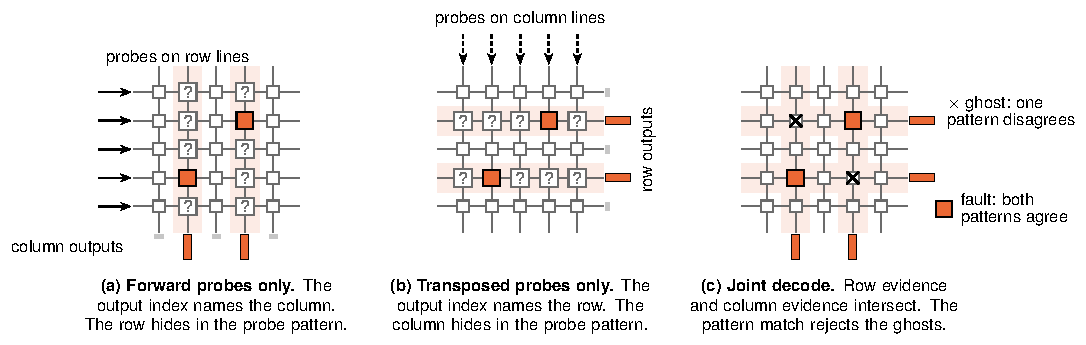
\includegraphics[width=\textwidth]{figs/fig_bidirectional.pdf}
\caption{Why two directions break the floor. The tile is drawn transposed relative to $W$: input lines are rows and output lines are columns. Two cells are faulty. (a) A forward read flags the two output columns but not their rows. (b) A transposed read flags the two rows but not their columns. (c) The joint decode intersects both sets. Four cells are candidates. Two are ghosts: one direction's pattern does not match.}
\label{fig:bidir}
\end{figure*}

\subsection{What we can prove}
\label{sec:proof}
We prove a sufficient condition (App.~\ref{app:proof}) and argue one identifiability fact. We do not prove that two directions need fewer reads than one.

\begin{lemma}[Cells in different rows and columns are orthogonal]\label{lem:orth}
Let $\varphi_{ij}$ be the joint-operator atom of cell $(i,j)$. Then $\langle\varphi_{ij},\varphi_{i'j'}\rangle=[i=i']\langle a_j,a_{j'}\rangle+[j=j']\langle b_i,b_{i'}\rangle$. Two cells that share no row and no column are exactly orthogonal.
\end{lemma}

Only same-row pairs (through the forward reads) and same-column pairs (through the transposed reads) interact. Let $S$ be the fault set and $\psi$ a normalized atom. Define $a=\max_{\psi\notin S}\sum_{\varphi\in S}|\langle\psi,\varphi\rangle|$ and $a'=\max_{\varphi\in S}\sum_{\varphi'\in S\setminus\varphi}|\langle\varphi,\varphi'\rangle|$. Lemma~\ref{lem:orth} bounds both by the number of faults that share a row or column with a cell.

\begin{proposition}[Sufficient condition]\label{prop:suff}
Assume: white Gaussian noise with known $s$; an exact linear model with no quantization and no drift during the probes; probes drawn independent of $E$; $a'<1$ and $a+a'<1$; and $|E_{ij}|\ge\delta$ on $S$. Let $\nu=p_f/n+p_b/m$, $b=\sqrt{2\ln(2mn/\eta)}$ and $\kappa=1+\max(a,a')/(1-a')$. If
\begin{equation}
\frac{\delta\sqrt{\nu}}{s}>\frac{2\kappa b}{1-a-a'},
\end{equation}
then orthogonal matching pursuit with stopping threshold $\kappa b$ recovers $S$ exactly with probability at least $1-\eta$.
\end{proposition}

The proof adapts the exact-recovery condition of Tropp \cite{tropp2004} and the noise analysis of Cai and Wang \cite{caiwang2011} (App.~\ref{app:proof}). We state its limits.
\begin{itemize}
\item It is a sufficient condition and it is not tight. At the registered minimum visible amplitude $\delta=0.1\max|w|$, it needs more than the 256 reads of a full readout at every noise level, so it gives no guarantee there.
\item It is about exact support recovery. It gives no guarantee on F1 $\ge0.9$, which allows missed cells.
\item It does not describe the shipped decoder. The shipped decoder uses a smaller threshold ($\kappa=1$) and a final prune. The proposition covers a more conservative variant.
\item It does not cover non-white or drifting noise, ADC/DAC quantization, a wrong noise estimate, or an inexact reference.
\item It is not a like-for-like comparison with Wei and Roth. Their guarantee is deterministic, for bounded noise and output-level localization in one MVM. Ours is probabilistic, for Gaussian noise and cell-level localization.
\end{itemize}
As a consistency check, take $k=1$ and the idealized constants $a=a'=0$, $\kappa=1$, $\delta=0.88\max|w|$ (the median visible deviation) and $\eta=0.1$. Condition (1) then needs 3.7, 14.9 and 59.6 reads at 1\%, 2\% and 4\% noise. We measured 4, 16 and 64 reads (Table~\ref{tab:loc}). The $\sigma^2$ scaling of 1:4:16 holds exactly.

\textbf{One fault, no noise.} With forward reads only, the output index names one coordinate. The other coordinate must come from the vector $E_{ij}a_j\in\mathbb R^{p_f}$, which has to tell $n$ candidates apart. With $\pm1$ probes, a counting argument over sign patterns gives $p_f\ge\log_2 n+1=9$ reads with the best $\pm1$ design, and about 16 with random probes; real-valued (multilevel-DAC) probes are not covered by this argument. With both directions, one forward read names the output line and one transposed read names the input line, so two reads suffice. The two-read statement is an achievability illustration for $k=1$ without noise, not a lower bound, and App.~\ref{app:proof} does not prove it.

\textbf{Why this is not an advantage theorem.} The worst-case incoherence term of the joint design is up to 2$\times$ \emph{worse} than forward-only when each line holds the same number of faults.
The measured advantage at low noise (1.5 to 3.7$\times$ fewer reads at 1\% noise, Sec.~\ref{sec:results-b})
An average-case bound on ghost cells would turn it into a theorem. We did not prove one.

\subsection{Concurrent regression from live inputs}
\label{sec:a8}
\textbf{Setup (H7, registered before the full run).} Each $256\times256$ tile gets two analog checksum lines programmed with the same noise as the weights: $c_1=\sum_i \W_{0,i}$ and $c_w=\sum_i \tfrac{i+1}{m}\W_{0,i}$, each scaled to the full conductance range and read back with its gain. Every inference MVM then yields two syndromes $s_1=\sum_i y_i-g_1y_{c_1}$ and $s_w$. A commissioning step right after programming (128 passes over 2048 fault-free inputs) fits the checksum lines' programming mismatch and the noise scale. All methods see the whitened residuals. We store no digital outputs. Live inputs are the cached im2col vectors of each layer. Faults are stuck cells injected after programming. Read noise is 2\%. We use 3 seeds $\times$ 8 conv layers $\times$ 4 tiles.
Methods: \textbf{CK} (our adaptation of the Neural Checksums / HPE detection rule, whose originals compare exactly in the digital domain): energy of the $s_1$ residuals, threshold at 1\% false alarms. \textbf{HPE decoder} (the weighted/plain ratio decoder of HPE and X-ABFT \cite{liu2020xabft}): the syndrome ratio over flagged samples names the faulty output row. \textbf{A8} (ours; the two checksum lines and the ratio decoder are prior art, the combination below is what we study): orthogonal matching pursuit of the $s_1$ residuals on the whitened inputs across $T$ inferences, Bonferroni stop at 1\% false alarms per tile. It returns faulty \emph{input} lines.

\subsection{Few-probe field-fit calibration (\mfour{})}
\label{sec:m4}
\textbf{Model.} Let $\W_0\in\mathbb R^{m\times n}$ be the stored digital reference of a tile's programmed weights and $A(t)$ the aged
array. Patterned drift is multiplicative, $A(t)-A(t_c)\approx\W_0\circ F$ (not low-rank even when $F$ is smooth, which is why a low-rank fit of the error does not work),
with $F=\sum_{a,b<4}c_{ab}\,\varphi_a(i)\varphi_b(j)$ and $\varphi_a(i)=\cos(\pi a(i+\tfrac12)/m)$ (\emph{cosine basis, order 4}: 16 coefficients per tile).

\textbf{Probes.} At calibration time $t_c$ (right after programming) read $Y_0=A(t_c)X$ with $X\in\{\pm1\}^{n\times 8}$ and $Z_0=A(t_c)^{\!\top}Z$ with $Z\in\{\pm1\}^{m\times 7}$,
and store $Y_0,Z_0$ digitally. At recalibration time $t$, re-read the same probes, form $\Delta Y=A(t)X-Y_0$ and $\Delta Z=A(t)^{\!\top}Z-Z_0$. Both are linear in $c$:
$(\W_0\circ\varphi_{ab})X$ and $(\W_0\circ\varphi_{ab})^{\!\top}Z$. A ridge least-squares solve (ridge $10^{-8}$ of the mean Gram diagonal) uses $8m+7n=3840$ scalars to fit 16 unknowns.
The corrected effective operator is $A(t)-\W_0\circ\hat F$ (\emph{ideal} form).
\textbf{Ideal versus deployable.} The ideal form needs the stored digital $\W_0$ at every inference: it is a digital MVM per tile, so it serves only as an upper reference for what the field \emph{estimate} is worth.
The \emph{deployable} form multiplies the analog array by $G=1/(1+\hat F)$ projected on the $4\times4$ cosine span and truncated to rank $r$ by SVD, $\sum_{k\le r}\mathrm{diag}(u_k)\,A(t)\,\mathrm{diag}(v_k)$: each term is one analog pass with digital input/output scaling, so rank 1 is free and the full form (rank $\le4$) costs up to 3 extra passes per inference (Sec.~\ref{sec:phaseh}).
One further read of the stored layer-mean input vector gives a digital bias correction (the same bias step is given to the \bviii{} baselines).
\textbf{Cost.} 8 forward $+$ 7 backward probes $+$ 1 bias read $=16$ MVMs per tile per recalibration (the \emph{strict} budget);
the variant run in Exp.~2 and first run in \texttt{a\_bnfold} uses 8 $+$ 8 probes plus the bias read $=17$. Zero calibration images are needed.

\textbf{Incumbent \bviii{}.} The strongest cheap digital baseline: per tile, the best of \{global GDC, per-row gain, per-column gain, bi-scale
$\mathrm{diag}(a)\W_0\mathrm{diag}(b)$\} (each fitted from 8 probe reads) plus the same mean-bias correction, \emph{selected per tile by its output error against the programmed weights on held-out activations}.
This oracle-style selection is optimistic for the incumbent (Sec.~\ref{sec:threats}).
% =================================================================================================
\section{Experimental Setup}
\label{sec:method-sim}
\subsection{Simulator}
Tiles are $256\times256$ blocks of the flattened conv weights of a trained ResNet-9 (109 tiles per network; blocks with a side $<16$ dropped).
Weights are encoded as differential pairs: $|w|$ on one device (G$^+$ for positive, G$^-$ for negative weights), the other at $g_{\min}=0.01\,g_{\max}$,
with tile-abs-max scaling and $g_{\max}=25\,\mu$S. Programming noise, drift and read noise use constants \emph{read from the installed AIHWKit 1.1.0 source}
\cite{rasch2021,rasch2023} (``sourced'' in Table~\ref{tab:params}); the spatial structure of drift and the temperature model have no
measured source and are ``assumed'' and swept.
Device $(i,j)$ evolves as $G(t)=G_0\big((t+t_0)/t_0\big)^{-\nu_{ij}}$ with $t_0=20$\,s;
\emph{D2} draws $\nu\sim\mathcal N(\mu(g),\sigma(g))$ per device from the AIHWKit PCM model; \emph{D3} adds a position-dependent field,
$\nu_{ij}=|\mu(g)+\sigma(g)(z_{ij}+\rho f_{ij})|$ with $f$ unit-variance (row gradient, rank-$r$ cosine, or Gaussian hotspot), so $\rho$ is the
structured-to-iid ratio and $\rho=0$ reproduces D2 exactly; \emph{D4} adds an Arrhenius time-acceleration and a read-gain temperature field (all assumed).
Probe reads are white per-cell noise of $\sigma_c=2\%$ of the tile's $\max|w|$, fresh on every MVM. This is the AIHWKit 1/f model's value
for trained ResNet-9 tiles (2.0\% rms, 2.6\% p90, 4.5\% at $g_{\max}$ at $t=20$\,s; 2.4\% rms at 1\,d), treated as uncorrelated across reads.
Network accuracy is evaluated in \emph{weight space}: the decoded, drifted, corrected effective weights replace the conv weights in PyTorch (BN folded, digital bias).
No ADC/DAC quantization is applied to the probe reads in the headline runs.

\begin{table}[t]
\caption{Provenance of simulator constants (full registry: \texttt{src/neurofault/spectral/params.py}, dumped to \texttt{params.json} in every run dir).}
\label{tab:params}
\centering\footnotesize
\begin{tabular}{p{2.5cm}p{1.9cm}p{3.0cm}}
\toprule
Constant & Status & Value / source \\
\midrule
PCM $\mu(g),\sigma(g)$ of $\nu$ & sourced & $\mu=\mathrm{clip}(-0.0155\ln g_r+0.0244,\,0.049,\,0.1)$; $\sigma=\mathrm{clip}(-0.0125\ln g_r-0.0059,\,0.008,\,0.045)$; AIHWKit \\
$t_0$ & sourced & 20\,s (AIHWKit) \\
1/f read noise & sourced & $q_s=\min(0.0088/g_r^{0.65},0.2)\sqrt{\ln\frac{t+t_r}{2t_r}}$, $t_r=250$\,ns \\
Programming noise & sourced & AIHWKit coefficients $[0.26348,1.9650,-1.1731]$ \\
Pattern strength $\rho$ & \textbf{assumed} & sweep $\{0,.25,.5,1,2,4\}$; no measured spatial correlation of $\nu$ found \\
Field shapes, hotspot width, rank $r$ & \textbf{assumed} & width 0.2$\max(m,n)$, $r=2$ \\
Temperature (D4): $E_a$, $T$, $\beta$, $\Delta T$ & \textbf{assumed} & 0.5\,eV, 330\,K, $10^{-3}$/K, 20\,K \\
Energy/latency constants & \textbf{assumed} & not used for any headline claim \\
\bottomrule
\end{tabular}
\end{table}

\subsection{Counted-read model}
Every method touches a tile only through a reader that counts reads: a forward MVM of $p$ vectors adds $p$ to \texttt{mvm\_fwd} (and $mp$ ADC conversions, $np$ DAC drives),
a transposed MVM adds $p$ to \texttt{mvm\_bwd}, a full cell readout adds $mn$ cell reads. In this paper a backward MVM costs one MVM
(backward-read cost is hardware-unverified). AdaBS cost is images $\times$ per-layer patch positions, in MVM-equivalents. A full-network recalibration of \mfour{} costs
$109\times16=1744$ MVMs (strict) or $109\times17=1853$ (as run) %
versus 2,622,312 for AdaBS-256 and 26,624,872 for AdaBS-2600 (E2/pareto\_W1.csv).
\emph{The inference-time cost of applying the correction is not counted; see Sec.~\ref{sec:threats}.}
\textbf{What the localization read counts include.} Counted reads in Table~\ref{tab:loc} cover the \texttt{localize()} call only. The 8 forward reads that estimate the read-noise level are excluded for every method, and the decoder is given the cap $2k+4$ (Sec.~\ref{sec:a5}). Including the 8 calibration reads would raise every count in the tables by 8, which matters most for the joint decoder at 4 to 12 reads; we did not re-run the registered ratios with that charge, so the 4.3 to 6.4$\times$ factor is stated without it.

\subsection{Pre-registration protocol}
\label{sec:protocol}
Each claim is a YAML file of clauses. A clause has a metric, a filter, an aggregation, a comparator and a threshold, and the file has a \texttt{frozen} date. A script (\texttt{verdict.py}) computes each status: PASS, NOT\_MET, KILL, CLEAR, INCONCLUSIVE or REPORTED. Each \texttt{verdict.json} stores the SHA-256 of the criteria file it used. A threshold may change only in a new commit with a logged reason. The log has two entries: a YAML parsing bug (\texttt{1.0e4} read as a string) and a check we had transcribed against the wrong circuit. Neither entry changed a threshold on the data.
A \emph{registered follow-up} is allowed only if the failed claim stays on record. \texttt{a\_bnfold} (after Exp.~2) and \texttt{b\_c1b} (after the C1 kill) were registered \emph{after} the result that suggested them. \texttt{a\_hardening} was registered before its run (H2). Follow-ups use fresh random streams (seed offsets $+1000$, $+2000$, $+4000$, $+5000$) and are listed next to the failure that motivated them (Table~\ref{tab:ledger}).
Fresh randomness is not a fresh checkpoint. \texttt{a\_bnfold} reuses the CIFAR-10 checkpoints (seeds 42/101/102); only the CIFAR-100 checkpoints are new. Smoke runs never count.

\subsection{Methodology and rigor}
\label{sec:honest}
A result that no one tried to break is weak. We used five practices.

\textbf{1. We registered first and let a script judge.} Phase H, the closed loop X, its extension, E4 and E5 had their criteria committed before their counted runs. Commits: 6ade20d (H2), 37af453 (H5), a9a1928 (H6, H2b), d6bc34d (H7), 35a83d3 (H8) and 018276a (E4, E5). For E4 and E5 the counted runs began 11 and 12 minutes after the commit.
For every registered follow-up and every Phase H file, the commit that adds the criteria file precedes the start time of the run it judges. We checked this with \texttt{git log}. Commit times are the only independent timestamps.

\textbf{2. We disclose the late first wave.} The criteria for F0, Gate~0$'$, Exp.~2 and the first B claims (C1, E1) were committed in 8c2ab18, after nine full runs. The commit message says so. Their thresholds were fixed in plans committed earlier (8cb7364). We did not diff the YAML against the plan text. So the repository cannot prove that these thresholds predate the data.

\textbf{3. We re-ran the competitors on their terms.} E4 tuned X-ABFT per row. E5 ran Wei and Roth's decoder under bounded noise. We froze the E4 and E5 criteria after a smoke run of 2 instances on 1 checkpoint. That run had shown that the one-MVM Wei--Roth decoder flags no line at 1 to 4\% noise, and that X-ABFT reaches F1 0.0 to 0.66 at 4\% even with 16 repeats. So two outcomes (E5 own-terms NOT\_MET and E4 noise degradation PASS) were foreseeable. We set the thresholds by what would change a paper claim, and we print the outcomes as they came.

\textbf{4. We report what failed.} The 21 criteria files end as follows: 4 PASS, 7 KILL, 10 INCONCLUSIVE (overall verdict of the final counted run of each file; \texttt{a\_bnfold} is counted under its strict 16-MVM reading, and under the as-run 17-MVM reading it is INCONCLUSIVE, giving 3 PASS, 7 KILL and 11 INCONCLUSIVE).
The kills include two of our own registered claims about transposed reads (C1, C1b), the $\sigma_1$ watchdog, the analog eigen loop, the free in-array form of \mfour{}, and the closed-loop extension at 4\% noise. Table~\ref{tab:ledger} lists 19 of the 21 files with their mechanical outcomes, and Table~\ref{tab:limits} lists 21 limits.

\textbf{5. We audited the raw data.} We recomputed all 52 verdict files from the stored metrics. 46 reproduce exactly. The other six are smoke runs (four) or killed variants without a stored metrics file (two), and no counted verdict differs. For 40 of 44 run directories, the code commit does not reproduce the run tree, because the scripts were first committed in 2ac6e07, after those runs. The stored configuration hashes and checkpoint SHA-256s identify the inputs, but the code state of those runs is not archived.

\begin{table*}[t]
\caption{Pre-registration ledger: every registered claim of the vertical that this paper touches, with its mechanical outcome. Follow-ups are listed directly below the claim that motivated them.}
\label{tab:ledger}
\centering\footnotesize
\begin{tabular}{p{2.6cm}p{1.5cm}p{9.2cm}p{2.9cm}}
\toprule
Claim (criteria file) & Frozen & Outcome & Run dir \\
\midrule
Validity gates F0.0a--e & 10-08 & all PASS: AIHWKit D2 distribution match (KS $p=0.023>0.01$, mean-ratio error 0.003), legacy-drift parity (max diff 0), invariants. & f0\_0/\allowbreak 20261008T204618\_e55b3002\_s0 \\
H1 bridge F0.8a--c (\texttt{f0\_validity}) & 10-08 & F0.8c PASS (no-drift accuracy within the binomial CI, 0.53 half-widths); F0.8a \textbf{NOT\_MET} (twin vs CrossSim max 5.66\pt, bar 0.5; mostly \bviii{} in BN-folded/hotspot cells); F0.8b \textbf{NOT\_MET} (twin vs AIHWKit native 1.34\pt, bar 1.0). & f0\_8/\allowbreak 20261011T151445\_d931ec73\_s0 \\
Gate 0$'$ (\texttt{a\_gate0}) & 10-08 & G0-a PASS (B8 excess error 4.0\,pp), G0-d PASS (oracle-16 vs B8 3.0\pt{}); G0-b NOT\_MET (specificity 0.095 $<0.15$), G0-c NOT\_MET, G0-e NOT\_MET (M1 partial AUC 0.60), G0-f NOT\_MET (Jacobian rank deficit 1). Frozen rules: GK-drop-C2 KILL, GK-relabel REDIRECT. & a\_gate0/\allowbreak 20261009T020655\_ae67b976\_s0 \\
F0.1 stuck cells vs $\sigma_1$ & 10-08 & H1.1 PASS (AUC$<$0.6 in 99.4\% of cells); H1.2 NOT\_MET (exponents $-1.40$, $+0.81$); H1.3-line NOT\_MET (AUC 0.69). & f0\_1/\allowbreak 20261009T023921\_a8f8370e\_s0 \\
F0.3 headroom, watchdog & 10-08 & H3.2 PASS, H3.3 PASS, H3.5 CLEAR; H3.4 KILL ($\sigma_1$ watchdog); H3.1 NOT\_MET (strict per-seed ordering; seed 101 within evaluation noise). & f0\_3/\allowbreak 20261009T181003\_aca2558e\_s0 \\
Exp.~2 (\texttt{a\_success}) & 10-08 & S1 PASS; S2 not met (stored verdict INCONCLUSIVE, see text); K1/K2/K4 CLEAR; overall INCONCLUSIVE. & a\_exp2/\allowbreak 20261009T052819\_52891c48\_s0 \\
\quad $\hookrightarrow$ \texttt{a\_bnfold} (BF1--3) & 10-09 & Strict 16 MVM: \textbf{PASS} on all five. As run (17 MVM): BF3 NOT\_MET $\Rightarrow$ INCONCLUSIVE. & a\_bnfold\_v2/\allowbreak 20261010T022159\_fca882d8\_s0 \\
B claim C1 (\texttt{b\_claims}) & 10-08 & C1 NOT\_MET (0/5 $k$ qualify) $\Rightarrow$ C1-kill \textbf{KILL}. & b\_c1\_prereg/\allowbreak 20261009T035140\_0fdb78ed\_s0 \\
\quad $\hookrightarrow$ \texttt{b\_c1b} & 10-09 & C1b-128 PASS (5/5 $k$); C1b-256 NOT\_MET (0/5) $\Rightarrow$ C1b-kill \textbf{KILL}; tile 512 reported 1/5. & b\_c1b/\allowbreak 20261009T115059\_609a698a\_s0 \\
C$'$ analog loop (\texttt{c\_claims}) & 10-08 & S1 NOT\_MET, K1a KILL, K1b KILL (median SNR ratio 0.24), D1 KILL. & c\_x1/\allowbreak 20261010T023044\_1e4807e2\_s0 \\
H2 stronger baselines, ideal \mfour{} (\texttt{a\_hardening}) & 10-10 & NI vs HB1$_8$, HB1$_{32}$, HB2, HB3 all PASS; kill not fired. Upper reference only (ideal form needs digital $\W_0$). & a\_hardening/\allowbreak 20261010T220159\_8434d92b\_s0 \\
H5 deployable cost (\texttt{a\_deploy}) & 10-10 & H5-deploy NOT\_MET; free rank-1 variant \textbf{KILL} (paired-CI lower bound $<0$ at every CIFAR-100 time). & a\_deploy/\allowbreak 20261010T223102\_71522b22\_s0 \\
\quad $\hookrightarrow$ H2b deployable \mfour{} (\texttt{a\_hardening\_deploy}) & 10-10 & NI vs HB2, HB3 PASS; NI vs HB1$_8$, HB1$_{32}$ NOT\_MET; kill and pairing gate CLEAR $\Rightarrow$ INCONCLUSIVE. & a\_hardening\_deploy/\allowbreak 20261011T041351\_794c47e8\_s0 \\
H8 CS vs prior-art localizers (\texttt{b\_vs\_prior}) & 10-11 & CS-2x, CS-4x, CS-forward-2x PASS; kill CLEAR $\Rightarrow$ \textbf{PASS}. & b\_vs\_prior/\allowbreak 20261011T210412\_0ec5ea78\_s0 \\
X closed loop, estimated map (\texttt{x\_loop}) & 10-12 & dense, edge, sparse, gap PASS; kill CLEAR $\Rightarrow$ \textbf{PASS}. & x\_loop\_box/results \\
X ext.\ (5 seeds, $\sigma$ 4\%, ViT-tiny) (\texttt{x\_loop\_ext}) & 10-12 & $\sigma$4, ViT PASS; R9 5-seed NOT MET (reads 0.2525 vs 0.25); kill FIRES (recall 0.85--0.89 vs 0.90 at $\sigma$ 4\% sparse) $\Rightarrow$ \textbf{KILL}; accuracy gap $\geq -0.07$\,pt every group. & x\_loop\_ext/results \\
H6 refresh allocation (\texttt{a\_refresh}) & 10-10 & saves-writes PASS; sensing-adds-value NOT\_MET; kill CLEAR (0.991 / 0.993 $<1$) $\Rightarrow$ INCONCLUSIVE. & a\_refresh/\allowbreak 20261011T185337\_449adbef\_s0 \\
H7 concurrent (\texttt{b\_concurrent}) & 10-11 & C5-detect, C5-locate, beats-HPE NOT\_MET; both kills CLEAR $\Rightarrow$ INCONCLUSIVE. & b\_concurrent/\allowbreak 20261011T152741\_d4b34e56\_s0 \\
E4 X-ABFT baseline (\texttt{e4\_xabft}) & 10-14 & E4-CS-2x PASS (4 of 4 $k$ at 1\% and at 2\%); E4-ratio-decode-degrades PASS (X-ABFT F1 $<0.9$ at 4\%, max 0.594); both kills CLEAR $\Rightarrow$ \textbf{PASS} (report scope INCONCLUSIVE by design).
 & e4\_xabft/\allowbreak 20261014T124345\_4b2720f4\_s0 \\
E5 Wei--Roth on its own terms (\texttt{e5\_weiroth\_fair}) & 10-14 & E5-own-terms \textbf{NOT\_MET} (line F1 0); E5-CS-2x-bounded PASS; E5-CS-2x-gauss PASS; both kills CLEAR $\Rightarrow$ INCONCLUSIVE as designed.
 & e5\_weiroth\_fair/\allowbreak 20261014T124416\_9b59bf83\_s0 \\
\bottomrule
\end{tabular}
\end{table*}

% =================================================================================================
\section{Results}
\label{sec:results}
\subsection{Fault localization: when two directions help}
\label{sec:results-b}
We start with the registered comparison against prior-art localizers (H8), then the two fair re-runs (E4, E5), and then the regime map where the second direction did not help (C1, C1b).

\subsubsection{Against prior-art localizers (H8, registered, PASS)}
Table~\ref{tab:loc} compares the HPE-style binary search, our Roth-style hybrid reimplementation of the Wei--Roth disjunct code (not the authors' code, and not the E5 decoder), and our joint compressed-sensing decoder with forward-only and with forward plus transposed probes. Every family's configuration is frozen on a calibration split (fault seeds 3000--3019, tile origin 1; selection rule as C1b) and evaluated on 240 fresh instances per cell (3 checkpoints $\times$ 4 layers $\times$ fault seeds 60--79). Registered bars: $\ge2\times$ and $\ge4\times$ fewer reads than Wei--Roth (paired-CI upper bound $\le0.6$ / $\le0.33$, or Wei--Roth misses F1 0.9 while CS reaches it) on $\ge3$ of 4 $k$ at each of 1\% and 2\% noise; both PASS, and so does the forward-only $2\times$ bar; kill CLEAR (median ratio 0.19).
The forward-only decoder passes its own registered bar too, so the comparison with the hybrid mostly measures the decoder and not the second direction (see the attribution below).
With both directions the decoder needs 4.3--6.4$\times$ fewer reads at 1\% and 5.1--5.4$\times$ at 2\% for $k\ge4$; a single fault at 2\% is the exception (16 vs 32 reads, 2.0$\times$, CI upper 0.52). At 4\% and $k\ge4$ our reimplementations of both prior-art schemes fall short of F1 0.9 (HPE-style 0.02--0.40, Wei--Roth-style 0.28--0.39) while the decoder reaches F1 0.93--0.95 with 32 reads.

\textbf{How much is the decoder and how much is the second direction.} Table~\ref{tab:loc} separates the two. The hybrid needs 26/27/51/51 reads at 1\% for $k=1/4/16/64$; forward-only compressed sensing needs 16/12/16/16, and the joint decoder 4/6/8/12. So the forward-only decoder alone already needs 1.6 to 4.1$\times$ fewer reads than the hybrid across 1--2\% noise, and the registered forward-only bar (H8-CSF-2x) passes. The second direction adds the rest at 1\% noise; at 2\% it adds nothing at $k=1$ (16 vs 16) and 1.3 to 2.0$\times$ in the other cells, and at 4\% it adds nothing for $k\ge4$ (32 vs 32) and costs reads at $k=1$ (64 vs 48).

\begin{table}[t]
\caption{H8, E4 and E5: mean reads of the frozen configuration on fresh faults (tile 256, 240 instances per cell); ``--'' = held-out cell F1 $<0.9$. Full readout = 256.}
\label{tab:loc}
\centering\scriptsize\setlength{\tabcolsep}{2.5pt}
\begin{tabular}{lccc}
\toprule
Method & 1\% & 2\% & 4\% \\
\multicolumn{1}{c}{} & \multicolumn{3}{c}{\scriptsize reads at $k{=}$1/4/16/64} \\
\midrule
HPE binary search & 10/--/--/-- & 39/--/--/-- & 157/--/--/-- \\
Roth-style hybrid (our reimpl.) & 26/27/51/51 & 32/41/65/--$^\ast$ & --/--/--/-- \\
Joint CS, forward only & 16/12/16/16 & 16/12/16/24 & 48/32/32/32 \\
Joint CS, both directions & 4/6/8/12 & 16/8/12/12 & 64/32/32/32 \\
Full cell readout (reference) & 256/256/256/256 & 256/256/256/256 & 256/256/256/256 \\
\midrule
X-ABFT, tuned (E4) & --/--/4096/2048 & --/--/--/-- & --/--/--/-- \\
Wei--Roth line, one MVM (E5) & --/--/--/-- & --/--/--/-- & --/--/--/-- \\
Wei--Roth cell, best (E5) & --/--/--/-- & --/--/--/-- & --/--/--/-- \\
\bottomrule
\end{tabular}
\par\smallskip{\scriptsize $^\ast$65 reads at F1 0.895. X-ABFT reaches F1 0.9 at 1\% noise only for $k=16$ and $64$ (F1 0.915, 0.936). Both E5 rows hold under bounded and under Gaussian noise; the line decoder's line F1 is 0.}
\end{table}

\subsubsection{X-ABFT, tuned per row (E4, registered, PASS)}
X-ABFT stores two checksum columns per block and decodes (row, column, deviation) from their ratio \cite{liu2020xabft}. We built a runnable version. We tuned its design and its repeat-and-average factor separately for every $(k,\sigma_c)$ row, on the same 240 instances per row as H8. The registered clause E4-CS-2x passes. On 4 of 4 $k$ at both 1\% and 2\% noise, the joint decoder needs at least 2$\times$ fewer reads than X-ABFT, or X-ABFT misses F1 0.9 while the decoder reaches it.
We print the F1 values next to the read counts, because the pass rests mostly on the second branch. At 1\% noise X-ABFT reaches F1 0.9 only for $k=16$ and $k=64$ (F1 0.915 and 0.936), with 4096 and 2048 reads against 8 and 12 for the decoder. For $k=1$ and $k=4$ its F1 is 0.667 and 0.822.
At 2\% noise X-ABFT never reaches 0.9 (F1 0.484 to 0.858).
Every tuned X-ABFT row at 1\% and 2\% noise uses 1024 or more reads, so it needs more reads than a full 256-read readout of the tile, including the two rows where it reaches F1 0.9 (4096 and 2048 reads).
At these fault counts the practical comparator is therefore a full readout and not X-ABFT. We ran no positive control: X-ABFT inside its own design regime (at most two faults per block, negligible noise) was checked only by unit tests with noise-free reads, not in the registered harness, so E4 cannot separate a stress test outside the design regime from a weak implementation.
The strict rule, a measured 2$\times$ on every row, holds on 2 of 4 $k$ at 1\% and on 0 of 4 at 2\%.
The second registered clause also passes. At 4\% noise X-ABFT stays below F1 0.9 for every $k$ (best 0.594), while the decoder reaches 0.93 to 0.95 for $k\ge4$. This turns ``the ratio decoder is noise-fragile'' from an expectation into a measurement.
Neither kill fired: X-ABFT never reached F1 0.9 with fewer reads than the decoder.

\textbf{Regime caveat.} X-ABFT is designed for at most two faults per block at 1 to 10\% fault density, with no per-read noise. Our regime is $k\le64$ faults in a $256\times256$ tile (about 0.1\% density) with Gaussian read noise. This run is a stress test outside its design regime. It is not a like-for-like benchmark, and we do not write ``X-ABFT fails''.
Three choices favor X-ABFT: its checksum lines come from the noise-free digital reference, its detection is noise-aware, and we gave it a repeat-and-average knob that its paper lacks.

\subsubsection{Wei and Roth on their own terms (E5, registered, INCONCLUSIVE as designed)}
Our H8 baseline (``Roth-style hybrid'' in Table~\ref{tab:loc}) is a hybrid (see the list below), so we also ran the Wei--Roth decoder as its paper defines it \cite{weiroth2024}: one MVM with $r$ redundant columns and a threshold on the syndrome. We ran it under bounded noise (rms-matched to the Gaussian noise) and under Gaussian noise, at 1, 2 and 4\% (240 instances per row). We froze the criteria in 018276a before the counted run.

\textbf{Own terms: NOT\_MET.} The one-MVM line decoder never reaches line F1 0.9. It flags no line: line F1 is 0 on every row (at most $1.3\times10^{-4}$), with 25, 49, 121 and 121 redundant columns for $k=1,4,16,64$.
Their guarantee needs outliers larger than $2\rho\delta\|x\|$. With our noise model the threshold grows with the probe norm, and the parity checks sum about 52 noisy lines, so it lies above our fault amplitudes (median visible deviation about 0.88 $\max|w|$, visibility floor 0.1 $\max|w|$). This explanation is our judgment from a smoke note, not a registered result: no clause evaluated the guarantee's constants. We call it a regime mismatch and not a failure of their method; their decoder behaves as specified in our unit tests (an outlier above $2\rho\delta$ is located, one below it is missed).

\textbf{Comparison clauses: PASS.} Forward-only decoding needs at least 2$\times$ fewer reads than the best Wei--Roth cell-level arm (PASS under our own pass rule), or the arm misses F1 0.9 while the decoder reaches it. This holds on 4 of 4 $k$ under bounded noise and on 3 of 4 $k$ under Gaussian noise, at both 1\% and 2\%. Under Gaussian noise at $k=4$ and 2\%, our decoder reaches F1 0.896, so that row fails.
All passes come from the second branch. No Wei--Roth cell arm reaches F1 0.9 on any 1--2\% row. The best arm reaches F1 0.38, 0.26, 0.11 and 0.17 at 1\% for $k=1,4,16,64$, and at most 0.016 at 2\%. So we did not measure a read ratio. We measured that these arms do not reach F1 0.9 on our faults. Neither kill fired.
The overall verdict is INCONCLUSIVE by design: the registered rule needs all clauses to pass, and a pass of the own-terms clause would have meant that their method works on our faults.

\textbf{Fairness of the Wei--Roth comparison.} Four points remain, and E5 removes none of (i) and (ii).
(i) The Wei--Roth paper stops at output lines. The cell-level stage of our H8 baseline is our own forward-only extension. So the baseline is a hybrid of their output-level stage and our input-side probe stage. The honest headline is cell-level localization against a hybrid group-testing baseline, not ``$\times$ fewer reads than Wei and Roth''.
(ii) Their cost unit is $r$ redundant columns inside one MVM. The reads in Table~\ref{tab:loc} are the cost of our reimplementation. The cost axes differ.
(iii) Their guarantees are for bounded noise. Under Gaussian read noise at 1 to 4\% our reimplementation needs thresholds and repeats, a regime the authors did not design for.
(iv) Our registered pass rule credits a Wei--Roth failure to reach F1 0.9, which counts failures outside their noise model as wins.
What we print is this. Under bounded and under Gaussian noise, no Wei--Roth arm we built reaches F1 0.9 in our fault regime, and the one-MVM line decoder detects nothing because the outliers sit below its guarantee.

\subsubsection{When the second direction does not help (C1 and C1b, both killed)}
\textbf{Setup.} Localize $k\in\{1,2,4,8,16\}$ stuck cells in a tile with \emph{counted} reads at cell-level F1$\ge0.9$; compare the best bidirectional design
(forward $A\mathbf x$ plus transposed $A^{\!\top}\mathbf y$ reads) against the best forward-only design (A1--A7, including HPE-style binary search and a Wei--Roth-style code; our reimplementations),
with identical tuning effort. Configs are frozen on a calibration split and evaluated on held-out faults (3 checkpoints $\times$ all conv layers, 20 fault seeds in C1; 20 fresh seeds in C1b).
No ADC or DAC quantization (\texttt{adc\_bits=None}); read noise $\sigma_c\in\{1\%,2\%\}$ of $\max|w|$ (1\% is optimistic-PCM/pessimistic-ReRAM, 2\% the AIHWKit PCM central value; Sec.~\ref{sec:method-sim}).
\textbf{C1 (pre-registered): KILL.} Reads ratio $\le0.7$ with CI upper bound $\le0.8$ and F1$\ge0.9$ for $\ge3$ of 5 $k$.
The reads ratio held out of sample on 29 of 30 rows (0.28--0.75), but the frozen bidirectional configuration's held-out F1 fell just below 0.9 (0.857--0.899) on at least one row for every $k$: 0/5 qualify.
Supplementary per-tile-size evaluation of the same criterion: tile 128 and 256 PASS, tile 512 NOT\_MET (C1/verdict\_tile*.json).
\textbf{C1b (registered after the kill): KILL} (Table~\ref{tab:c1b}, Fig.~\ref{fig:ratio}). Margin-calibrated selection (calibration F1$\ge0.93$), tiles 128 and 256 only (scope chosen \emph{after} tile 512 failed; disclosed), fresh fault seeds. Tile 128 PASS 5/5; tile 256 0/5 (reads, not accuracy:
at $\sigma_c=2\%$ the bidirectional design needs 12 reads vs 16 for forward-only, ratio 0.75 $>0.7$). The margin fixed generalization (held-out F1 $\ge0.9$ on 29/30 rows).

\begin{table}[t]
\caption{C1b reads ratio (bidirectional / best forward-only) at F1$\ge0.9$, fresh fault seeds. Entries marked $^\dagger$ fail the registered row test (F1$\ge0.9$, ratio $\le0.7$, CI upper $\le0.8$). Bar: 0.7.}
\label{tab:c1b}
\centering\footnotesize
\begin{tabular}{llccccc}
\toprule
Tile & $\sigma_c$ & $k{=}1$ & 2 & 4 & 8 & 16 \\
\midrule
128 & 1\% & 0.27 & 0.33 & 0.49 & 0.50 & 0.67 \\
128 & 2\% & 0.50 & 0.50 & 0.50 & 0.50 & 0.67 \\
256 & 1\% & 0.42 & 0.50 & 0.38 & 0.38 & 0.50 \\
256 & 2\% & 1.00$^\dagger$ & 0.75$^\dagger$ & 0.75$^\dagger$ & 0.75$^\dagger$ & 0.75$^\dagger$ \\
512 & 1\% & 0.38 & 0.38 & 0.38 & 0.50 & 0.50 \\
512 & 2\% & 1.00$^\dagger$ & 0.67$^\dagger$ & 1.00$^\dagger$ & 1.00$^\dagger$ & 0.67 \\
\bottomrule
\end{tabular}
\end{table}

\begin{figure}[t]
\centering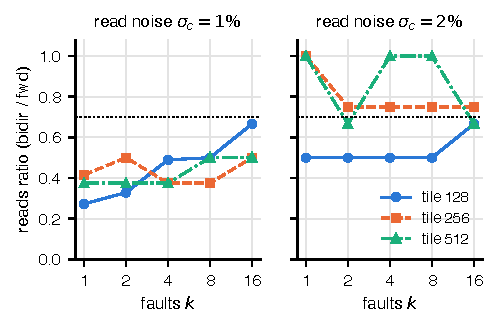
\includegraphics[width=\columnwidth]{figs/fig_reads_ratio.pdf}
\caption{Reads ratio versus fault count at 1\% (left) and 2\% (right) read noise. Dashed: the registered 0.7 bar. The advantage is real at 1\% on every tile size and disappears at 2\% on tiles $\ge256$.}
\label{fig:ratio}
\end{figure}

\textbf{What survives as a finding, not a claim.} At $\sigma_c=1\%$ bidirectional reads need 1.5--3.7$\times$ fewer reads on every tile size (ratios 0.27--0.67, typically 2--3$\times$); at the PCM-typical 2\% the saving is 1.5--2$\times$ on tile 128 and marginal or absent on 256 and 512 (ratios 0.67--1.0).
\emph{Selection optimism is visible in our own history}: an exploratory run (best-of selection on the evaluation instances, 2 layers $\times$ 5 seeds) reported a 2.0$\times$ saving (12 vs 6 reads) at $k{=}1$, tile 256, 2\% noise; the same cell on fresh seeds shows 16 vs 16 reads (ratio 1.0).
Two further regime facts: with random $\pm1$ probes and a generic joint decoder the two-direction advantage vanishes by about 16 reads (L9; scratch numbers, not a registered result), and probing beats a full 256-read readout of a 256$\times$256 tile only up to a fault density of 0.3\%
(\texttt{probing\_win\_max\_density}=0.003; at $\ge1\%$ full readout wins), far below the 10\% per-wave density of repair campaigns, where localization by probing is not worth its reads.
The ``estimated map drives repair'' claim (C4) is out of scope here.

\subsubsection{Ways to localize stuck cells, and what each costs}
\label{sec:tradeoff}
Several of these methods localize stuck cells, and they differ in what hardware and decoding they need, not only in reads.
Table~\ref{tab:tradeoff} collects the numbers above for one representative fault count, $k=16$ in a $256\times256$ tile, and adds the requirements and the regime where each method is the better choice.

\begin{table*}[t]
\caption{Ways to localize stuck cells, and what each costs. Reads are means at $k=16$ stuck cells (tile 256) from Table~\ref{tab:loc}; ``--'' means held-out cell F1 $<0.9$ (HPE-style F1 0.11--0.12; X-ABFT at 2\% reaches F1 0.832 with 4096 reads). Every arm here uses the stored digital weights as reference. Decoder compute is a qualitative judgment, not a measurement. ``Best choice'' states a regime, not a ranking, and is limited to the tile size, noise grid and stuck-at fault model we tested.}
\label{tab:tradeoff}
\footnotesize
\begin{tabular}{@{}>{\raggedright\arraybackslash}p{2.4cm}>{\raggedright\arraybackslash}p{1.2cm}>{\raggedright\arraybackslash}p{1.2cm}>{\raggedright\arraybackslash}p{1.3cm}>{\raggedright\arraybackslash}p{1.3cm}>{\raggedright\arraybackslash}p{2.6cm}>{\raggedright\arraybackslash}p{5.0cm}@{}}
\toprule
Method & Reads, 1\% noise & Reads, 2\% noise & Transposed reads? & Stored digital weights? & Decoder compute & Regime where it is the best choice \\
\midrule
Full readout & 256 & 256 & No & Yes & None (subtract) & Fault density above about 0.3\% (exploratory, tile 256), or when a robust answer is needed whatever the noise \\
HPE-style binary search & -- & -- & No & Yes & Very low & Not the best in our grid; it reaches F1 0.9 only at $k=1$ (10 reads at 1\%, 39 at 2\%), where a forward-only decoder is not available \\
Roth-style hybrid (our reimpl.) & 51 & 65 & No & Yes & Low (threshold and group test) & Not the best in our grid; its published guarantee is for bounded noise and outliers above its threshold, and our fault amplitudes sit below it (E5) \\
X-ABFT, tuned (E4) & 4096 & -- & No & Yes & Low (ratio decode) & Its design regime, at most two faults per block at 1--10\% density with negligible read noise, which we did not test in the registered harness \\
Forward-only sparse decode & 16 & 16 & No & Yes & Moderate (sparse recovery) & Default when the array cannot be read transposed, or at 2--4\% noise; it reaches or nearly reaches F1 0.9 on every row of the grid (0.900 at 2\%, $k=4$) \\
Joint (forward + transposed) sparse decode & 8 & 12 & Yes & Yes & Moderate to high (larger operator) & Low noise (1\%) on a transposable array, where it needs half the reads of forward-only; at 4\% and $k\ge4$ it gives no gain \\
\bottomrule
\end{tabular}
\end{table*}

Which method to choose depends on the noise, the fault density and the array.
Forward-only sparse decoding is the robust default: it needs no transposed read path, and it reached or nearly reached F1 0.9 on every row of our grid with 12 to 48 reads (F1 0.900 at 2\% and $k=4$).
Transposed reads pay only at low noise: at 1\% the joint decoder needs 8 reads against 16 at $k=16$, and at 2\% 12 against 16, and at 4\% with $k\ge4$ it needs no fewer.
Above about 0.3\% fault density a full readout of the tile is cheaper than probing, so it wins in the dense regime (an exploratory finding at tile 256).
The prior-art arms are not shown to be poor methods: each is outside its design regime here (E4 and E5 above), and the table is a statement about our fault model and read-noise grid.

\subsection{Concurrent localization from live inputs}
\label{sec:concurrent}
The setup of H7 is in Sec.~\ref{sec:a8}.
\textbf{Results} (Table~\ref{tab:h7}). The planned budgets (detect within 64 MVMs, localize within 256) are out of reach for every concurrent method: summing 256 cells' read noise on a checksum line leaves a per-inference SNR of about 0.05 (L21). The registered verdict is INCONCLUSIVE: the C5-detect, C5-locate and beats-HPE clauses were all NOT\_MET. Read from the report-level curves (Table~\ref{tab:h7}), with thousands of inferences A8 does better than our adaptations of the per-inference decoders: detection 0.99 vs 0.13 for CK at 16k inferences, and line F1 0.83--0.87 vs about 0.01 for the HPE decoder, whose row estimate needs ratio precision $1/(2m)$. False alarms on fault-free tiles were 0.4--1.2\% (A8). Almost no input line is dead (median dead fraction 0), so faults are observable from live data. 16k inferences of one tile are 64 images at the median layer (16 to 1024 by layer).
Dedicated tests that pause inference are cheaper for detection: 8 stored natural test inputs or 8 random $\pm1$ probes detect 16 stuck cells with power 0.98--1.00 (1 cell: 0.38--0.46).

\begin{table}[t]
\caption{H7: concurrent methods vs number of live inferences $T$ (min over seeds for detection; mean F1 over instances).}
\label{tab:h7}
\centering\scriptsize\setlength{\tabcolsep}{2.5pt}
\begin{tabular}{lccccc}
\toprule
$T$ & 64 & 256 & 1024 & 4096 & 16384 \\
\midrule
Detect 1 big fault, CK & 0.04 & 0.06 & 0.09 & 0.11 & 0.13 \\
Detect 1 big fault, A8 & 0.05 & 0.15 & 0.60 & 0.92 & 0.99 \\
Line F1, HPE decoder ($k{=}4$) & 0.00 & 0.01 & 0.01 & 0.01 & 0.01 \\
Line F1, A8 ($k{=}4$) & 0.03 & 0.11 & 0.35 & 0.70 & 0.87 \\
Line F1, A8 ($k{=}1$ / $16$) & .03/.03 & .10/.09 & .39/.27 & .71/.60 & .86/.83 \\
\bottomrule
\end{tabular}
\end{table}


\subsection{Drift compensation}
\label{sec:results-a}
\subsubsection{Gate 0$'$: what failed}
The pre-registered gate asked four questions before any network-level work.
(i) \emph{Headroom} exists: the best cheap incumbent leaves 4.0\,pp more output error than at $\rho=0$ (G0-a PASS) and an oracle rank-16 correction would add 3.0\pt{} accuracy (G0-d PASS).
(ii) \textbf{Structure-specificity failed.} The original claim was that gains come from tracking drift \emph{structure}; the registered test required the capture gap between structured and iid drift to be $\ge0.15$, and measured 0.095 (G0-b NOT\_MET).
Figure~\ref{fig:gate0} shows why: \mfour{} already beats \bviii{} by 2.4\,pp output error at $\rho=0.25$ (sigma 2\%) and the gap grows to 12--14\,pp at $\rho=4$ for hotspot and rank-$r$ fields,
i.e.\ it is a better calibrator at every structure level, not a structure tracker. Under the frozen rule (GK-relabel) the vertical continues only as \emph{calibration-cost reduction}.
(iii) The \emph{watchdog} idea (dominant-mode statistics as drift classifier/trigger) failed: M1 partial AUC given the free GDC factor is 0.60 ($<0.7$, G0-e) and temperature, drift and aging are not separable (Jacobian rank deficit 1, G0-f); frozen rule GK-drop-C2 fired (KILL).
(iv) Realizable-over-oracle capture at 2\% probe noise was negative (G0-c NOT\_MET, $-2.2$ vs bar $0.6$); noisy-probe \mfour{} still beat \bviii{} on tile errors, and we did not investigate the metric further; the registered clause is NOT\_MET.
Caveats: reduced grid (1--2 tiles per layer), 1000-image evaluations, best-of per tile on both sides.

\begin{figure}[t]
\centering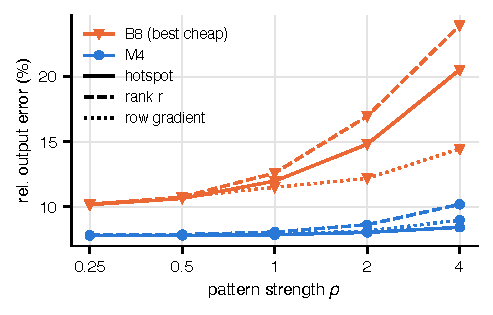
\includegraphics[width=\columnwidth]{figs/fig_gate0.pdf}
\caption{Gate 0$'$: relative output error of the best cheap incumbent (B8, orange) and field-fit M4 (blue) versus pattern strength $\rho$ for three field shapes (read noise 2\%).
M4 is ahead already at $\rho=0.25$ and the gap grows with $\rho$.}
\label{fig:gate0}
\end{figure}

\subsubsection{Exp.~2: \mfour{} versus AdaBS}
Table~\ref{tab:exp2} and Fig.~\ref{fig:exp2} give the network-level comparison (3 seeds, 2500 eval images, 2\% probe noise, PCM, 1\,h/1\,d/30\,d/1\,yr; pooled over the scenarios on which every listed method was run: D2 and D3-hotspot $\rho{=}1$).
\emph{With BN kept (W1)}, \mfour{} (87.29\%) beats \bviii{} (86.12\%, $+1.17$\pt, CI $[0.67,1.87]$; S1 PASS) but is $0.61$\pt{} below AdaBS-2600 (87.90\%; CI $[-1.21,+0.30]$),
and AdaBS-256 alone (87.58\%) is already within $0.25$--$0.39$\pt{} of AdaBS-2600 at one tenth of the cost, so there is no ``10$\times$ cheaper than AdaBS'' story: that saturation belongs to AdaBS.
Stacking \mfour{} on AdaBS-256 adds $+0.32$\pt{} over AdaBS-2600 (CI $[0.04,0.70]$) at 2.6M MVM-eq.
\textbf{S2 (match AdaBS-2600 within 0.3\pt{} at $\le1/10$ cost on $\ge2$ devices) was not met} (L16): the stored mechanical verdict reads INCONCLUSIVE because the S2 clause found no rows (the script did not emit the device column and only PCM was run); read by hand from \texttt{s2\_per\_scenario.csv}, no \mfour{} variant alone is within 0.3\pt{} of AdaBS-2600 (gaps 0.53--0.88\pt); the stacked \mfour{}+AdaBS-256 (one tenth of the cost) is within 0.3\pt{} on 2 of 4 scenarios; and only one device was evaluated.
\emph{With BN folded (W2)}, AdaBS is not applicable, GDC reaches 80.58\% and \bviii{} 81.42\%, while \mfour{} reaches 86.83\% ($+5.41$\pt{} over \bviii{}, CI $[3.75,7.08]$), equal to the programmed network (86.64\%).
That workload was the pre-registered motivation for \texttt{a\_bnfold}, which was registered \emph{after} seeing this number and is reported next to the S2 miss.

\begin{table}[t]
\caption{Exp.~2: accuracy and calibration cost (MVM-equivalents per whole network), mean over 3 seeds, 4 times and 2 scenarios. CI: paired bootstrap of the difference to \bviii{}.}
\label{tab:exp2}
\centering\footnotesize
\begin{tabular}{lrrr}
\toprule
Method & Cost & W1 (BN kept) & W2 (BN folded) \\
\midrule
GDC & 872 & 85.32 & 80.58 \\
\bviii{} & 985 / 982 & 86.12 & 81.42 \\
\mfour{} (8+8 probes + bias, 17 MVM/tile) & 1853 & 87.29 & 86.83 \\
AdaBS-256 & 2.62M & 87.58 & n/a \\
AdaBS-2600 & 26.6M & 87.90 & n/a \\
\mfour{}+AdaBS-256 & 2.62M & 88.22 & n/a \\
programmed (oracle) & --- & 87.73 & 86.64 \\
\bottomrule
\end{tabular}
\end{table}

\begin{figure}[t]
\centering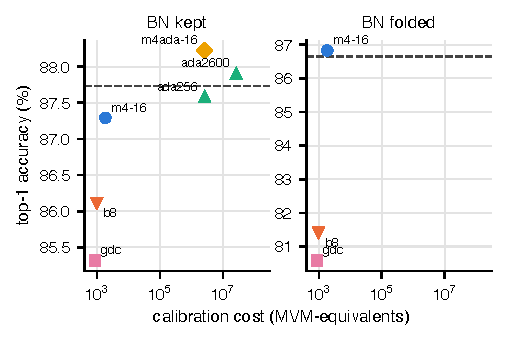
\includegraphics[width=\columnwidth]{figs/fig_exp2_pareto.pdf}
\caption{Exp.~2 accuracy versus calibration cost. Dashed: programmed network. With BN kept, AdaBS buys its last 0.6\pt{} with $10^3$--$10^4\times$ more MVMs than \mfour{}; with BN folded only \mfour{} (and cheap baselines) apply.}
\label{fig:exp2}
\end{figure}

\subsubsection{\texttt{a\_bnfold}: BN-folded deployment, registered follow-up}
\textbf{Registration.} Platform: ResNet-9 with BN folded; D2, D3 \{hotspot, rank-$r$, row-gradient\} at $\rho\in\{1,2\}$ (6 scenarios) and D4: 8 scenarios; CIFAR-10 and CIFAR-100, 3 checkpoint seeds each; $t\in\{1\text{h},1\text{d},30\text{d},1\text{yr}\}$; $\sigma_c=2\%$; 10k test images; streams offset $+1000$.
Claims: BF1 median $|$gap to programmed$|\le0.5$\pt; BF2 gain over \bviii{} $\ge2.0$\pt{} with paired-CI lower bound $>0$ at $\ge3$ of 4 times, per dataset; BF3 $\le16$ calibration MVMs per tile;
kills: BF-noharm (mean gain on iid drift $<-0.3$\pt) and BF-kill (CI lower bound $\le0$ at every time).
\textbf{Budget readings.} Three readings exist and are reported together: (a) \emph{strict 16}: 8 fwd $+$ 7 bwd $+$ 1 bias $=16$ MVMs total; (b) \emph{as run, registered count}: 16 field-fit probes counted, with the bias read as in the baselines (script convention);
(c) \emph{as run, counting the bias read}: 17 total. Table~\ref{tab:bf} and Fig.~\ref{fig:drift} show the outcome per time point, Table~\ref{tab:scen} per scenario, and Table~\ref{tab:bfverdict} the mechanical verdicts.

\begin{table*}[t]
\caption{\texttt{a\_bnfold} final: top-1 accuracy (\%), mean over 8 scenarios $\times$ 3 checkpoint seeds, 10k images. Gain = \mfour{} $-$ \bviii{}; CI lo = lower end of the 95\% paired cluster bootstrap CI (clusters = 3 checkpoints). Strict = 8+7+1 MVMs; as run = 8+8 probes + bias read.}
\label{tab:bf}
\centering\footnotesize
\begin{tabular}{llrrrrrr}
\toprule
 & & & \multicolumn{3}{c}{Strict (16 MVM)} & \multicolumn{2}{c}{As run (17 MVM)} \\
\cmidrule(lr){4-6}\cmidrule(lr){7-8}
Dataset & $t$ & Prog. & \mfour{} & \bviii{} & Gain [CI lo] & \mfour{} & Gain [CI lo] \\
\midrule
CIFAR-10 & 1\,h & 86.83 & 86.93 & 84.85 & $+2.08$ [1.08] & 86.58 & $+1.73$ [1.01] \\
CIFAR-10 & 1\,d & 86.83 & 86.99 & 82.19 & $+4.81$ [3.03] & 86.46 & $+4.28$ [2.50] \\
CIFAR-10 & 30\,d & 86.83 & 86.68 & 78.66 & $+8.03$ [5.84] & 86.83 & $+8.18$ [6.03] \\
CIFAR-10 & 1\,yr & 86.83 & 86.96 & 73.70 & $+13.27$ [9.93] & 86.76 & $+13.07$ [9.81] \\
CIFAR-100 & 1\,h & 48.54 & 47.74 & 47.20 & \textbf{$+0.53$ [$-$0.26]} & 48.55 & $+1.35$ [0.81] \\
CIFAR-100 & 1\,d & 48.54 & 49.04 & 44.81 & $+4.22$ [3.18] & 48.73 & $+3.92$ [2.43] \\
CIFAR-100 & 30\,d & 48.54 & 48.24 & 41.18 & $+7.06$ [5.53] & 49.06 & $+7.89$ [6.09] \\
CIFAR-100 & 1\,yr & 48.54 & 48.60 & 37.85 & $+10.75$ [8.76] & 48.61 & $+10.76$ [8.68] \\
\bottomrule
\end{tabular}
\end{table*}

\begin{figure}[t]
\centering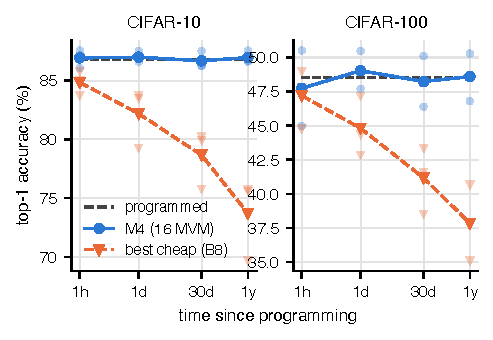
\includegraphics[width=\columnwidth]{figs/fig_drift_accuracy.pdf}
\caption{BN-folded ResNet-9 under simulated PCM drift (mean of 8 scenarios $\times$ 3 checkpoints). M4 tracks the programmed network (dashed) from 1\,h to 1\,yr; the best cheap compensation falls 13.1 (CIFAR-10) and 10.7 (CIFAR-100) points below programmed accuracy at 1\,yr.}
\label{fig:drift}
\end{figure}

\begin{table*}[t]
\caption{Mechanical verdicts of \texttt{a\_bnfold.yaml} under the three budget readings (values: C10 / C100).}
\label{tab:bfverdict}
\centering\footnotesize
\begin{tabular}{p{0.9cm}p{4.5cm}ccc}
\toprule
 & Value & Strict 16 & As run, count 16 & As run, count 17 \\
\midrule
BF1 & median gap to programmed (pt) & PASS ($-0.09$/$-0.20$) & PASS (0.13/$-0.14$) & PASS \\
BF2 & time pts (of 4) clearing gain $\ge2$, CI$>0$ & PASS (C10 4,4; C100 3,3) & PASS (C10 3,4; C100 3,4) & PASS \\
BF3 & MVMs per tile & PASS (16) & PASS (16) & \textbf{NOT\_MET} (17) \\
noharm & mean gain on iid D2 (pt) & CLEAR (+3.81/+3.23) & CLEAR (+3.57/+3.45) & CLEAR \\
kill & max CI lo over times (pt) & CLEAR (9.93/8.76) & CLEAR (9.81/8.68) & CLEAR \\
\midrule
Overall & & \textbf{PASS} & PASS & \textbf{INCONCLUSIVE} \\
\bottomrule
\end{tabular}
\end{table*}

\textbf{Reading.} The headline passes only under the strict 16-MVM budget; if one insists on counting the bias read for the as-run variant the registered BF3 is not met and the verdict is INCONCLUSIVE.
BF2 passes with exactly the allowed fraction (0.75) on CIFAR-100: the 1\,h point misses 2\pt{} on both datasets under the as-run variant, and under the strict variant CIFAR-100 at 1\,h has a gain of $+0.53$\pt{} whose CI includes zero.
Honest summary: from 1\,d to 1\,yr the effect is large and unambiguous; at 1\,h it is small and, for CIFAR-100, not distinguishable from zero.
\mfour{} also helps on iid drift ($+3.2$ to $+3.8$\pt), which is consistent with Gate 0$'$: the gain is not specific to structure. The H5 ablation (CIFAR-10, 1\,d and 1\,yr, all scenarios and seeds, report only) isolates the mechanism: in the ideal form even an order-1 field (one coefficient) from forward probes only reaches 85.2\% / 85.0\% (programmed 84.9\%, \bviii{} 83.0\% / 76.4\%), and order 4 or transposed probes add at most 1.1\pt. The ideal correction's strength therefore comes from using the stored digital $\W_0$ as the reference, not from the field's richness or the read direction; in the free rank-1 deployable form all orders stay at 75.6--78.1\% at 1\,yr.

\begin{table}[t]
\caption{Strict-variant gain over \bviii{} (pt) per scenario, mean over 3 seeds and 4 times.}
\label{tab:scen}
\centering\footnotesize
\begin{tabular}{lrr}
\toprule
Scenario & CIFAR-10 & CIFAR-100 \\
\midrule
D2 (iid, sourced PCM) & 3.81 & 3.23 \\
D3 hotspot $\rho{=}1$ / $2$ & 7.31 / 10.88 & 4.70 / 7.22 \\
D3 rank-$r$ $\rho{=}1$ / $2$ & 5.78 / 11.66 & 4.89 / 9.97 \\
D3 row-gradient $\rho{=}1$ / $2$ & 5.78 / 6.22 & 5.12 / 5.51 \\
D4 (temperature, assumed) & 4.92 & 4.50 \\
\bottomrule
\end{tabular}
\end{table}


\subsection{Deployability, stronger baselines and refresh (Phase H)}
\label{sec:phaseh}
\label{sec:h2}
Four registered runs (Table~\ref{tab:ledger}) test what the \mfour{} estimate is worth in hardware. All use the \texttt{a\_bnfold} platform with fresh streams and, from H5 on, activation statistics from augmented \emph{training} images only (this removes the test-image overlap of \bviii{}'s selection, Sec.~\ref{sec:threats}).

\textbf{Baselines (H2, registered before any run).} HB1: digital per-output-channel gain and bias from $N\in\{8,32\}$ augmented training images (the closest analogue of AdaBS for a folded network); HB2: per-column affine from reference columns \cite{ibm11663458}; HB3: offline-trained rank-4 adapters switched by a timer \cite{vera2026}.
Non-inferiority: scenario-mean difference $\ge-0.3$\pt{} at $\ge3$ of 4 times per dataset. The \emph{ideal} \mfour{} is non-inferior to all four (H2: all NI PASS), but that comparison only says the estimate is good.

\textbf{H5: the deployable form recovers much less.} The free rank-1 form gains $+0.1$ to $+1.5$\pt{} over \bviii{} (C10: $+0.89,+0.10,+1.46,+0.65$; C100: $+0.41,+0.88,+1.37,+0.25$ at 1\,h/1\,d/30\,d/1\,yr) with a paired-CI lower bound below zero at every CIFAR-100 time: the registered free-variant kill fired (L19).
Reprogramming every tile recovers everything (86.2\% C10, 48.9\% C100 at 1\,yr; one write per device per refresh).

\textbf{H2b: deployable \mfour{} against the baselines} (paired with H2: same streams, baseline rows reused; pairing gate 0.00\pt). Table~\ref{tab:h2}. The full deployable form is non-inferior to HB2 and HB3 at every time on both datasets and beats \bviii{} by 0.6--3.7\pt, but a digital recalibration from 32 images is 1.0--4.9\pt{} better from 1\,d on (8 images: up to 3.2\pt{} better, tied at CIFAR-100 30\,d): \mfour{} is \emph{competitive among image-free, weight-free methods}, not best.

\begin{table*}[t]
\caption{H2/H2b: top-1 accuracy (\%), mean over 8 scenarios $\times$ 3 checkpoints, 10k images. \mfour-d = deployable \mfour{} (rank-1 free; full = up to 3 extra analog passes per inference). Ideal \mfour{} needs digital $\W_0$ at inference (upper reference).}
\label{tab:h2}
\centering\footnotesize
\begin{tabular}{lp{2.6cm}cccccccc}
\toprule
 & & \multicolumn{4}{c}{CIFAR-10} & \multicolumn{4}{c}{CIFAR-100} \\
\cmidrule(lr){3-6}\cmidrule(lr){7-10}
Method & Cost per recalibration & 1\,h & 1\,d & 30\,d & 1\,yr & 1\,h & 1\,d & 30\,d & 1\,yr \\
\midrule
No correction & 0 & 49.31 & 24.29 & 14.48 & 12.56 & 16.25 & 3.98 & 1.58 & 1.17 \\
HB3 timer adapters & 0 reads, trained offline & 84.74 & 82.23 & 77.28 & 72.31 & 46.61 & 42.14 & 34.93 & 29.13 \\
HB2 reference columns & reference columns per tile & 85.21 & 82.87 & 78.66 & 74.04 & 45.89 & 43.24 & 38.31 & 33.31 \\
\bviii{} (optimistic) & 8 MVM/tile & 84.54 & 82.47 & 78.52 & 74.80 & 45.85 & 43.70 & 39.80 & 34.06 \\
\mfour-d rank 1 & 16 MVM/tile, 0 extra passes & 84.94 & 82.48 & 77.49 & 72.46 & 46.69 & 43.63 & 38.79 & 33.65 \\
\mfour-d full & 16 MVM/tile, $\le3$ extra passes & 85.14 & 83.21 & 79.87 & 76.48 & 46.96 & 44.55 & 41.70 & 37.75 \\
HB1, 8 images & 8 images & 85.49 & 84.19 & 81.97 & 79.72 & 47.59 & 45.42 & 41.68 & 38.27 \\
HB1, 32 images & 32 images & 85.94 & 84.88 & 83.15 & 81.40 & 47.77 & 45.80 & 42.70 & 39.80 \\
\midrule
\mfour{} ideal (needs digital $\W_0$) & 16 MVM/tile + digital MVM & 86.58 & 86.31 & 86.41 & 86.29 & 48.83 & 48.73 & 49.20 & 49.21 \\
\bottomrule
\end{tabular}
\end{table*}

\textbf{H6: \mfour{} as a refresh scheduler.} Since reprogramming recovers everything, the remaining use of the estimate is deciding \emph{which} tile to reprogram and \emph{when}. Registered model: each tile is refreshed at its own period from a 12-point age grid, chosen by a cost-weighted allocation from a health estimate (\mfour: predicted output error from 16 MVMs; GDC: drift-gain magnitude, 8 MVMs; STATIC: one nominal age curve, no sensing; ORACLE: the true error). Writes are per cell per year at equal worst-case network accuracy (Table~\ref{tab:h6}).
Any per-tile cost-aware allocation saves 99.6\% of the writes of a uniform timer at the 1-day target (91.6\% at the 30-day target, where every policy needs about one write per cell per year), because small tiles are cheap to refresh; \mfour's sensing saves a further 9--13\% of writes over STATIC at a 1-day target (median per-scenario ratio 0.87 and 0.91; bar 15\%, NOT\_MET) and nothing at 30 days, where every policy needs about one write per cell per year (L20). The medians in Table~\ref{tab:h6} are medians of writes, not of per-scenario ratios, and so imply larger savings (for example 1.61 against 2.07 on CIFAR-10).

\begin{table}[t]
\caption{H6: writes per cell per year to match a uniform timer's worst-case accuracy (median over 3 seeds $\times$ 8 scenarios).}
\label{tab:h6}
\centering\footnotesize
\begin{tabular}{lcccc}
\toprule
 & \multicolumn{2}{c}{CIFAR-10} & \multicolumn{2}{c}{CIFAR-100} \\
\cmidrule(lr){2-3}\cmidrule(lr){4-5}
Policy & 1-day & 30-day & 1-day & 30-day \\
\midrule
Timer & 365 & 12.2 & 365 & 12.2 \\
GDC allocation & 2.44 & 1.03 & 3.46 & 1.01 \\
STATIC (no sensor) & 2.07 & 1.01 & 4.44 & 1.01 \\
\mfour{} allocation & 1.61 & 1.02 & 2.91 & 1.01 \\
Oracle allocation & 1.52 & 1.02 & 2.25 & 1.01 \\
\bottomrule
\end{tabular}
\end{table}

% =================================================================================================
\section{Discussion and Limitations}
\label{sec:discussion}
\subsection{What survived and what did not}
A few counted probe reads tell a controller a lot about an aging crossbar. What limits their value is what the controller can do with them.

\textbf{What survived.}
(i) The joint decoder localizes tens of stuck cells in about a dozen reads at 1--2\% noise, given the stored digital weights and an otherwise ideal tile. For $k\ge4$ it needs 4.3 to 6.4$\times$ fewer reads than our hybrid reimplementation of a published multi-outlier code at 1\% noise (registered PASS under our own pass rule), most of it owed to the decoder, since the forward-only form already needs 1.6 to 4.1$\times$ fewer. It needs at least 2$\times$ fewer reads than tuned X-ABFT, or X-ABFT misses F1 0.9 (registered PASS, with regime caveats). At 4\% noise and $k\ge4$ it reaches F1 0.93 to 0.95 where our reimplementations of the baselines do not. This last comparison is report-level, not a registered clause, and it does not hold at $k=1$.
(ii) The drift estimate is accurate. The ideal (digital) correction restores programmed accuracy, and the health estimate correlates 0.98 with the true tile error.
(iii) Concurrent regression on ordinary inputs reaches detection 0.99 and line F1 0.83 to 0.87 at 16k inferences, where our adaptations of per-inference checksum decoders do not. This is report-level; the registered H7 verdict is INCONCLUSIVE with all three pass clauses NOT\_MET.

\textbf{What did not survive.}
The extra benefit of transposed reads over forward-only decoding is limited to small tiles or low noise, and two registered claims about it were killed (C1, C1b). We have no theorem for it. In the array, without stored digital weights, the drift correction is competitive among image-free methods but loses to a few-image digital recalibration. As a refresh scheduler, sensing saves a further 9 to 13\% of writes over a sensorless cost-aware schedule (median per-scenario ratio 0.87 and 0.91 at a 1-day target; bar 15\%, NOT\_MET).

\textbf{Open.} A proof of the advantage at low noise (an average-case bound on ghost cells). A decoder that works within 64 to 256 live inferences. Any result on real hardware or on faults other than stuck-at.
Table~\ref{tab:ledger} lists 19 of the 21 criteria files with their mechanical verdicts, including those that were killed or not met. The two not listed (F0.2 and F0.5) include no kill. The F0.5 V6p check is INCONCLUSIVE.

\subsection{Hand-off to the closed loop}
The tools that survive (the field estimate, the sparse-recovery decoder in its forward-only form, concurrent regression) are the inputs to the closed-loop repair work. A first registered closed-loop test (X.1/X.2, \texttt{criteria/x\_loop.yaml}, PASS) supports that hand-off: a remap-and-retrain controller acting on a fault map estimated from counted probe reads (the forward-only compressed-sensing decoder with 24 dense Rademacher probes and an OMP cap of 64, a full-readout fallback and 8 calibration reads charged per tile, 2\% read noise; the bidirectional decoder is not used in this loop) matched its own oracle-map accuracy within 0.25\,pt on ResNet-9 (3 seeds; 27\% stuck cells, and a sparse $\approx$0.3\% regime where the decoder used 0.23--0.25$\times$ the reads of full readout). The registered accuracy bars were $-1.0$\,pt (dense) and $-0.5$\,pt (sparse) mean gap. The observed gap ($\le$0.25\,pt) is the size of the run-to-run noise of the oracle itself (0.24\,pt), so this is a no-difference-detected result, not an equivalence test. In the dense regime the ``estimated'' map is largely the full-readout fallback (all 111 tiles in 4 of 5 waves), so only the sparse regime tests the efficient localizer. The dense oracle runs for seeds 42, 101 and 102 come from an earlier campaign on another machine, and the 0.25\,pt range does not extend to five seeds, where the dense gap ranges from $-0.42$ to $+0.24$\,pt.
A registered extension (5 seeds, 4\% read noise, ViT-tiny) kept the \emph{group-mean} accuracy gap within 0.3\,pt in every group (per-seed gaps from $-0.88$ to $+0.90$\,pt for ViT dense). It fired its pre-registered kill clause: at 4\% noise the worst wave of the sparse regime found only 85 to 89\% of the newly visible faults (bar 90\%), and one ResNet-9 seed used 0.2525$\times$ the reads (bar 0.25). Its details belong to the repair paper.

\subsection{Limits (L1--L21)}
\label{sec:limits}
The original motivation was an analog eigen loop pointed at the array's own matrix. The widely quoted ``about 10\% error at 10\% device variation'' for the Sun--Ielmini circuits belongs to the linear-system circuit \cite{sun2019pnas}, not the eigenvector one, so our loop simulator was checked against first-order eigenvector perturbation theory instead (registered V6p check in F0.5, median relative difference $5.6\times10^{-4}$; the F0.5 run is INCONCLUSIVE overall). Table~\ref{tab:limits} lists what we measured and why we do not build on it.
Evidence tiers: \textbf{R} = registered, mechanical verdict; \textbf{A} = analysis or proof; \textbf{S} = scratch numbers from a throwaway probe (re-implementation pending, treat as indicative).
Three measured scaling laws deserve emphasis: the shift of $\sigma_1$ from one stuck cell goes as tile size$^{-1.40}$ and $k^{+0.81}$ (theory $-1$ and $0.5$; H1.2 NOT\_MET, theory to be revised; F01); the eigenvector error under device variation scales as $1/\text{gap}$ (slope $-0.90$ on real tiles in the registered V6p run, band $[-1.3,-0.7]$; an earlier unregistered probe gave $-1.00$);
and the trained-weight spectral gap $\sigma_1/\sigma_2$ is only 1.02--1.11, which makes settling slow and the eigenvector ill-conditioned.
Figure~\ref{fig:s1} gives the main empirical picture: at 2\% noise the $\sigma_1$ shift is at chance for one fault on every tile size and only reaches AUC 0.60--0.92 at $k{=}64$ simultaneous faults (tile 512 down to tile 64),
while eight $\pm1$ probe reads already give AUC 0.72--0.89 for \emph{one} fault.

\begin{figure}[t]
\centering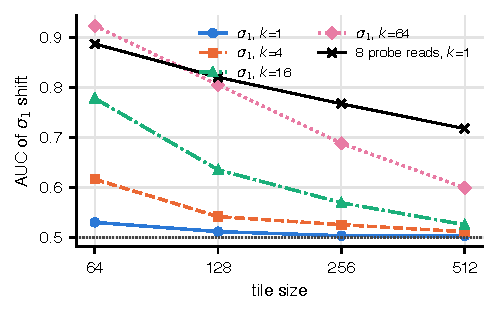
\includegraphics[width=\columnwidth]{figs/fig_sigma1_auc.pdf}
\caption{AUC of the dominant-singular-value shift as a stuck-cell detector versus tile size and fault count $k$ (2\% read noise, signed encoding; mean over layers/seeds), against eight $\pm1$ probe reads for $k{=}1$ (dashed).}
\label{fig:s1}
\end{figure}

\begin{table*}[t]
\caption{Limits L1--L21. Numbers are from the cited run directories; tiers as defined in the text.}
\label{tab:limits}
\centering\scriptsize
\begin{tabular}{p{0.5cm}p{3.9cm}p{8.8cm}p{0.5cm}p{2.5cm}}
\toprule
\# & Investigated & Finding & Tier & Source \\
\midrule
L1 & $\sigma_1$ as a fault signature & One stuck cell moves $\sigma_1$ by $\approx\delta/\sqrt{mn}$ (relative $\sim10^{-4}$), below read noise. AUC$<0.60$ in 99.4\% of (layer, tile, encoding, seed) cells at $k{=}1$, 2\% noise, max 0.59; identical for signed and G$^+$/G$^-$. Shift $\propto$ tile$^{-1.40}$, $k^{0.81}$. & R & f0\_1/\allowbreak 20261009T023921\_a8f8370e\_s0 \\
L2 & Self-check with no stored reference & Impossible: $\langle y,Ax\rangle=\langle A^{\!\top}y,x\rangle$ uses the same cells, so forward and backward reads always agree. & A & proof \\
L3 & Gain near the stability edge, shift-invert, deflation & Amplification is paid back in settling time or noise; shift-invert only guaranteed stable for positive-definite matrices. & A & research-01 \\
L4 & Rank-1 pilot to widen the gap & Fast settling, but the eigenvector shift is then a probe with $x=v_0$, i.e.\ a weighted checksum; scalar $\sigma_1$ stays blind (0\% at every $\beta$). & S & research-04 \\
L5 & Spectral gap of trained weights & $\sigma_1/\sigma_2=1.02$--$1.11$: slow loop settling, ill-conditioned eigenvector, noise-dominated ``mode-shape'' localization. & S & feasibility probe \\
L6 & Loop with hard-clipping amplifiers & All outputs latch to the rails at $\beta\ge3$; localization 0\%. Needs amplitude control. & S & scratch probe \\
L7 & ``Analog-only, no ADC'' as novelty & Already patented (HPE comparators on a syndrome; NVIDIA/Duke ADC-free power monitoring) \cite{hpe11804859,hpe11532356,nvidia11971790}. & A & literature \\
L8 & Uniform drift as evidence & Our first test (all cells $+5\%$ toward a rail) is an additive rank-1 change, near tautological; uniform multiplicative drift is fixed exactly by GDC. & A & research-02 \\
L9 & Random $\pm1$ probes, both directions & No two-direction advantage once reads reach about 16: information per read is symmetric. Gain needs structured designs. & S & scratch probe \\
L10 & Low-rank capture weighted by real inputs & Equal for random and patterned drift (inputs sit in few principal components); not evidence of drift structure. & S & scratch probe \\
L11 & Spectral/low-rank WATCH classifier & M1 partial AUC given GDC factor 0.60 ($<0.7$); temperature/drift/aging not separable (Jacobian rank deficit 1). Dropped by GK-drop-C2. & R & a\_gate0/\allowbreak 20261009T020655\_ae67b976\_s0 \\
L12 & Drift-structure-specific compensation & \mfour{} beats the best cheap incumbent at every structure level: specificity 0.095 $<0.15$. Gain is generic calibration. & R & a\_gate0 \\
L13 & Spectral detection of stuck lines & $\sigma_1$ AUC for a fully stuck line on tiles $\ge128$: 0.69 (H1.3-line NOT\_MET); a 1-row checksum matches within 0.006 AUC at 0.8\% of the cost. & R & f0\_1 \\
L14 & $\sigma_1$ ratio as drift watchdog & AUC 0.92 but only $+0.008$ over the free GDC-factor statistic (bar 0.05): H3.4 KILL. & R & f0\_3/\allowbreak 20261009T181003\_aca2558e\_s0 \\
L15 & Bidirectional localization, C1 & Reads ratio held out (0.28--0.75 on 29/30 rows) but F1 0.857--0.899: 0/5 $k$ qualify, KILL. & R & b\_c1\_prereg/\allowbreak 20261009T035140\_0fdb78ed\_s0 \\
L16 & Claim C1$'$: AdaBS accuracy at $\ge10\times$ fewer MVMs & \mfour{} 0.61\pt{} below AdaBS-2600 (CI $[-1.21,0.30]$); AdaBS-256 already near AdaBS-2600: S2 not met. & R & a\_exp2/\allowbreak 20261009T052819\_52891c48\_s0 \\
L17 & Follow-up C1b & Tile 128 PASS 5/5, tile 256 0/5, KILL. Bidirectional advantage real at 1\% noise (2--3$\times$), fades at 2\%. & R & b\_c1b/\allowbreak 20261009T115059\_609a698a\_s0 \\
L18 & Analog eigen loop as localizer & Registered: median SNR ratio 0.24 $<1/3$ against a $\pm1$ probe at equal output noise (K1b KILL), D1 KILL on 18 cells / 3 seeds. Unregistered plan-C probes (indicative only): settles in 0.05--0.19$\times$ one MVM when latch-free; signal 4--14$\times$ weaker than a probe; complex dominant eigenvalues on un-dilated tiles (50--100\% of tiles); never reaches 90\% localization at the probe's noise point; at probe-matched rail amplitude (c\_x1\_vt09) SNR ratio 0.45--0.57, localization 25--51\%, and the speed advantage disappears. Simulates the Sun-type leading-eigenvector loop, not the Mannocci $\lambda$-sweep circuit. & R & c\_x1/\allowbreak 20261010T023044\_1e4807e2\_s0; c\_x1\_vt09/ \\
L19 & \mfour{} applied in the array without digital $\W_0$ & Free rank-1 form: $+0.1$ to $+1.5$\pt{} over \bviii, CI lower bound $<0$ at every CIFAR-100 time (H5 kill). Full form ($\le3$ extra passes) beats HB2/HB3 but loses to 8--32-image recalibration. & R & a\_deploy/\allowbreak 20261010T223102; a\_hardening\_deploy/\allowbreak 20261011T041351 \\
L20 & \mfour{} health estimate as refresh allocator & Cost-aware allocation alone saves 99.6\% of timer writes at a 1-day target (91.6\% at 30 days); \mfour's sensing saves a further 9--13\% of writes over sensorless allocation at a 1-day target (median per-scenario ratio 0.87 and 0.91; bar 15\%, NOT\_MET), nothing at 30 days. & R & a\_refresh/\allowbreak 20261011T185337 \\
L21 & Concurrent detection/localization within 64--256 inferences & Per-inference checksum SNR $\approx0.05$ at 2\% noise; A8 detection 0.05 at 64 MVMs, line F1 0.06 at 256 (bars 0.99/0.9). Works at thousands of inferences (Sec.~\ref{sec:concurrent}). & R & b\_concurrent/\allowbreak 20261011T152741 \\
\bottomrule
\end{tabular}
\end{table*}

\subsection{Threats to Validity}
\label{sec:threats}
\textbf{Simulation only and the digital-twin bridge (H1).} Network accuracy is computed in weight space from our own device model; no silicon is used.
The registered bridge checks did not meet their agreement bars. No-drift accuracy matches the stored checkpoints (F0.8c PASS). Our drift + GDC against AIHWKit's native drift + GDC differs by up to 1.34\pt{} (F0.8b, bar 1.0). Pushing the \emph{same} corrected matrices through the repository's CrossSim system (8-bit DAC, calibrated 8-bit ADC) differs from the twin by up to 5.66\pt{} (F0.8a, bar 0.5); the large gaps are almost all on \bviii{} in BN-folded and hotspot cells (CrossSim is harsher on it), while \mfour{} agrees within about 2\pt.
On CrossSim the \mfour{}$-$\bviii{} gain of the \texttt{a\_bnfold} headline is \emph{larger} than in the twin ($+3.3/+6.8/+11.2/+16.7$\pt{} vs $+2.1/+4.7/+8.3/+13.2$ at 1\,h/1\,d/30\,d/1\,yr), so relative comparisons are conservative, but absolute accuracies are not validated to 0.5\pt.
A post-hoc diagnosis (report only; \texttt{f0\_8\_diag.py}) re-ran the 16 worst cells (BN-folded, seeds 101/102, D2 and hotspot, 1\,d and 1\,yr) on CrossSim at other converter resolutions: at 16-bit ADC and DAC CrossSim matches the twin to within 0.02\pt{} in every cell, so the twin computes the same network and the whole gap is converter quantization. Most of it comes from the 8-bit DAC (16-bit ADC with 8-bit DAC leaves 0.3--3.8\pt; 8-bit ADC with 16-bit DAC leaves $\le0.7$\pt), and it hits \bviii{} (2.5--4.8\pt) far harder than \mfour{} (0.6--1.6\pt).
\textbf{Localization idealizations.} The localizer uses the stored digital copy of the programmed weights, the test tile has no drift or programming noise, the noise level is estimated from 8 uncounted reads (charged in the closed loop), the decoder is given the cap $2k+4$, probes and decoder settings are tuned per $(k,\sigma_c)$ cell, read noise is white and independent across the forward and transposed reads of a cell, there is no ADC/DAC quantization, success is a mean F1 of 0.9 with no per-chip escape rate, and a transposed read assumes bidirectional periphery whose cost is unverified. Cell-persistent noise would correlate the two directions and weaken the second one. Statistics treat the 240 instances per cell as independent although they come from 3 checkpoints and 4 layers with 20 fault draws each.
\textbf{Inference-time cost of the correction.} Measured in H5/H2b (Sec.~\ref{sec:phaseh}): the ideal form costs a digital MVM per tile, the deployable full form up to 3 extra analog passes per inference, rank 1 nothing. The headline \texttt{a\_bnfold} numbers use the ideal form and are an upper reference.
\textbf{Counting of the probe budget.} 16 vs 17 MVMs (Table~\ref{tab:bfverdict}); backward reads are assumed to cost one MVM; reference reads $Y_0,Z_0$ are stored digitally (15 vectors per tile) and their capture at programming time is not charged to recalibration; a transposable array is required.
\textbf{Statistics.} Three checkpoint seeds per dataset, so the paired bootstrap resamples 3 clusters (its lower bound is a coarse guide); headline binomial standard error at 10k images is about 0.35\pt{} at 87\% accuracy.
\textbf{Incumbent selection and test-set reuse.} \bviii{} picks its best member per tile using the programmed weights as ground truth on held-out im2col activations built from the first 5000 CIFAR test images (the same images overlap the 10k evaluation set); the layer-mean input for the bias step comes from the same cache.
This favors the incumbent (a deployable \bviii{} would be worse), so it makes the reported gain conservative, but absolute accuracies of both arms may be slightly optimistic. From H5 on, every statistic comes from augmented training images.
\textbf{Absolute accuracy.} The as-programmed networks sit 1.3\pt{} (CIFAR-10) and 3.3\pt{} (CIFAR-100) below float (88.15\% and 51.87\% mean); \mfour{} restores programmed, not float, accuracy; programming error is out of scope.
\textbf{Scope.} One architecture (ResNet-9), 256$\times$256 tiles, PCM only for the headline (RRAM/CMO and FeFET paths exist in the simulator but have no network result); structured drift fields and temperature parameters are assumed; no ADC/DAC quantization (except the CrossSim tier of H1) and white (not 1/f-correlated) read noise. The localization results (Sec.~\ref{sec:results-b}, \ref{sec:concurrent}) use stuck-at faults only.
\textbf{Registration.} \texttt{a\_bnfold} and \texttt{b\_c1b} were registered after seeing the results that motivated them; they used fresh random streams but not fresh checkpoints (CIFAR-10) and, for C1b, a tile scope chosen after tile 512 failed.
The thin CIFAR-100 1\,h point and the two budget readings are reported rather than resolved.

% =================================================================================================
\section{Conclusion}
\label{sec:conclusion}
A deployed chip cannot re-read every cell, and one-sided probing has a floor it cannot pass. Reading the array from both sides removes that floor at low noise. In simulation, a joint decoder localizes up to 64 stuck cells in a $256\times256$ tile with 4 to 12 reads at 1\% read noise. For $k\ge4$ it needs 4.3 to 6.4$\times$ fewer reads than a hybrid reimplementation of a published code, and at least 2$\times$ fewer than tuned X-ABFT, or X-ABFT misses F1 0.9.
The advantage fades at 2\% noise on large tiles, and we prove only a sufficient condition. We pre-registered the criteria, disclosed the late first wave, ran the competitors on their own terms, and reported the failed ideas. The result that survived is narrow, and we state its limits.

\section*{Reproducibility}
Code, configurations, raw run records and analysis scripts: \url{https://github.com/prateek1656/NeuroFault}. Commit identifiers cited in this paper refer to the author's timestamped development repository, available to reviewers on request. Code: \texttt{src/neurofault/spectral/}, \texttt{experiments/spectral/} (e.g.\ \texttt{a\_bnfold.py}, \texttt{b\_c1b.py}); frozen criteria: \texttt{experiments/spectral/criteria/*.yaml}.
Every run directory holds \texttt{config.json}, \texttt{params.json}, \texttt{run\_metadata.json} (config hash, checkpoint SHA-256s, library versions) and \texttt{verdict.json}.
Figures: \texttt{scripts/figures/paper\_b/make\_figs.py} reads only committed CSVs, and \texttt{fig\_bidirectional.tex} is the TikZ source of Fig.~\ref{fig:bidir}.



\appendix[Proof sketch of Lemma~\ref{lem:orth} and Proposition~\ref{prop:suff}]
\label{app:proof}
\textbf{Lemma 1.} The atom of cell $(i,j)$ is $\varphi_{ij}=[\,e_i\otimes a_j\,;\,e_j\otimes b_i\,]$. Its forward block lives on the forward measurements of output line $i$ with pattern $a_j$. Its transposed block lives on the transposed measurements of input line $j$ with pattern $b_i$. The inner product of two atoms is the sum of a forward term and a transposed term. The forward term is zero unless $i=i'$, and then it is $\langle a_j,a_{j'}\rangle$. The transposed term is zero unless $j=j'$, and then it is $\langle b_i,b_{i'}\rangle$. $\square$

\textbf{Proposition 1 (sketch).} Normalize the atoms, $\psi=\varphi/\|\varphi\|$, and whiten the reads by $s$. Then $y=\Psi_S c+\varepsilon$ with $\varepsilon\sim\mathcal N(0,I)$ and $|c_{ij}|\ge c_{\min}=\delta\sqrt{\nu}/s$, because $\|\varphi_{ij}\|^2=\nu$. The event $G=\{\max_\psi|\langle\psi,\varepsilon\rangle|\le b\}$ has probability at least $1-\eta$ (Gaussian tail and a union over the $mn$ atoms). On $G$ we show by induction that matching pursuit picks only atoms of $S$. Suppose the chosen set $T\subset S$ and $T\ne S$. The residual is $u+\tilde n$ with $u=(I-P_T)\Psi_{S\setminus T}c$ and $\tilde n=(I-P_T)\varepsilon$.
(i) For every atom, $|\langle\psi,\tilde n\rangle|\le\kappa b$, because $\|G_T^{-1}\|_{\infty\to\infty}\le 1/(1-a')$.
(ii) On $S$: $\|\Psi_S^{\top}u\|_\infty\ge(1-a')c_{\min}$.
(iii) Off $S$: $|\langle\psi,u\rangle|\le\frac{a}{1-a'}\|\Psi_S^{\top}u\|_\infty$.
The best atom of $S\setminus T$ then beats every atom outside $S$ when $(1-a-a')c_{\min}>2\kappa b$. This is condition (1). It also exceeds the threshold $\kappa b$. When $T=S$, every correlation is at most $\kappa b$ and the procedure stops. The steps follow Tropp \cite{tropp2004} and Cai and Wang \cite{caiwang2011}. We checked Lemma~\ref{lem:orth} by hand. The proof of the proposition has not been independently reviewed.

\bibliographystyle{IEEEtran}
\bibliography{refs}

\end{document}
